 \hspace{0.5cm} 
 Our dataset consists of $N=2,613$ Spanish business news articles 
 sourced from DowJones and spanning the period from 2020/06/24 to 2021/09/30. 
 We denote as $\mathcal D$ the set of all articles in our sample.
 % from DowJones for the period 2020-6-24 to 2021-09-30. 
 These articles have been specifically filtered to reference firms listed on the IBEX-35.
% These articles have been specifically filtered to be explicitly referred to firms that are listed in the IBEX-35.
 Let $\F_{\t{IBEX35}}$ denote the universe of such firms. 
 Each article $i \in \mathcal{D}$ is a textual document detailing an event that directly pertains to a subset of firms $\mathcal{F}^i \subseteq \F_{\t{IBEX35}}$.
% Each article $i\in \D$ is a textual document narrating an event that directly involves a set of firms %$\F^i \subseteq \F_{\t{IBEX35}}$.
%
The publication date and time of each article are represented as $\mathcal{Y}_0^i = \langle d_0^i, t_0^i \rangle$, where $d_0^i$ captures the date 
(YYYY-MM-DD) 
and $t_0^i$ captures the time
 (HH:MM) 
 of publication. 
%This datetime representation emphasizes 
Therefore we observe
the moment at which $\mathcal{F}^i$ receives the \qquote{treatment} of public news dissemination. 
%The information conveyed by an article can then be represented in a tuple 
%$
%\langle i, \F^i , \mathcal Y_0^i \rangle 
%$

%The article is published at some datetime represented by a tuple $\mathcal Y_0^i :=\angl{d_0^i, t_0^i}$, where $d_0^i$ represents the date component (YYYY-MM-DD) and $t_0^i$ represents the time component (HH:MM:SS.SSS). We use a 0-subscript to emphasize that $\mathcal Y_0^i$ is the day and time in which $\mathcal F^i$  receives  ``treatment'' (publication of a news article directly involving $\mathcal F^i$).
%%``treatment date'' or day in which a news article is published regarding firm $j$ (firm $j$ receives treatment) 
%

\mx 
For robust model development and evaluation, the dataset is partitioned into three sequential subsets: training, validation, and test:
$
\D := \D^{tr} \cup \D^{val} \cup \D^{test}.
$
Define $N_{split}:=|\D^{split}|$ for $split\in\3{tr,val,test}$, where $\abs{\cd}$ denotes the cardinality of a set. 
%Then, it follows that
%%with $N_{tr}:=\abs{\D^{tr}}, N_{val}:=\abs{\D^{val}}$, N_{test}:=\abs{\D^{test}}$ 
%$\abs{\D}= N_{tr} + N_{val} + N_{test} = N$. 
%----------------------------------------------------
%The training and validation samples represent 80\% of the total sample $(\frac{N_{tr}+N_{val}}{N} = 0.8)$ and are used to design the optimal trading strategy, while the test sample represents the remaining 20\% $(\frac{N_{test}}{N} = 0.2)$ and is used to evaluate the \textit{out-of-sample} performance of the strategy. 
%--------- CHAT GPT OPTION ---------%
The training and validation sets collectively comprise 80\% of the total dataset $(\frac{N_{\text{tr}} + N_{\text{val}}}{N} = 0.8)$ and are instrumental in constructing and fine-tuning the trading strategy. The remaining 20\% $(\frac{N_{\text{test}}}{N} = 0.2)$ is reserved for out-of-sample testing to assess the performance and generalizability of the strategy under unseen conditions.
%----------------------------------------------------

%%%%%%%%%%%%%%%%%%%%%%%%%%%%%%%%%%%%%%%%%%%%%%%%%%%%%
%%%%%%%%%%%%%%%%%%%%%%%%%%%%%%%%%%%%%%%%%%%%%%%%%%%%%
\subsection{Publication datetime \& Effective treatment day}
\hspace{0.5cm} We are interested in examining the impact of each news article $i\in\D$ on the stock price of the firms that are affected directly (i.e.: all $j\in\F^i$). Since the publication datetime is not necessarily a trading datetime, we cannot directly gauge such an effect by looking at $\mathcal Y_0^i$. 
For this reason, we need to work through some definitions. 
%
%$(\tilde{d}_0^i)$ as the date at which news article $i$ events can be incorporated into the stock prices of $\F^i$. 
%
Let $\T$ denote the set of all datetimes in the sample timeline and let $\widetilde{\T}\subset \T$ be the subset of Spanish trading datetimes associated to our sample.
\begin{align*}
\widetilde{\T} := 
\3{\angl{d,t} \mid d \in \tilde{\mathfrak d} ~\wedge~ t\in \tilde{\mathfrak t}}
,
\end{align*}
where 
$
\tilde{\mathfrak{d}}:=\{\tilde{\mathfrak{d}}_{[1]},\tilde{\mathfrak{d}}_{[2]}, \ldots \tilde{\mathfrak{d}}_{[n]}\}
$
is the ordered set of week and non-festive days according to the Spanish calendar in our data timeline,
%, and $\tilde{\mathfrak t}$ are the trading hours 
and 
$\tilde{\mathfrak t}:=
\{t \mid \t{09:30} \leq t \leq  \t{17:30}\}
%\{t \mid t\in\t[\t{09:30}, \t{17:30}]\}
$
 are the Spanish stock market trading hours. 
Note that we use tildes to emphasize that we are considering trading dates or times. 

%We can now define a set of functions that will become useful as we work with trading days.
%We now introduce some functions that will prove useful now and later on for easily handling trading days. 

%%----------------------------------------------------
%
\textbf{Index Function}. 
Given a finite ordered set $\mathcal{Z}=\left\{z_1, z_2, \ldots, z_n\right\}$, the index function 
$\mathbb{I}_{\mathcal{Z}}: \mathcal{Z} \rightarrow\{1,2, \ldots,|\mathcal{Z}|\}$
%$\mathbb{I}_{\mathcal{Z}}(z)$
 maps an element $z\in\Z$ to its position in the ordered set $\mathcal{Z}$. Formally:
$$
\mathbb{I}_{\mathcal{Z}}(z_{\ell})=\ell 
%\quad \text { if and only if } \quad z=z_{\ell} 
\quad \text { for } \quad \ell \in\{1,2, \ldots,|\mathcal{Z}|\}
$$
%where $z_{\ell}$ denotes the ${\ell}$-th element of the ordered set $\mathcal{Z}$.

\textbf{Inverse Index Function}. 
The inverse index function 
$\mathbb{I}_{\mathcal{Z}}^{-1}:\{1,2, \ldots,|\mathcal{Z}|\} \rightarrow \mathcal{Z}$
%$\mathbb{I}_{\mathcal{Z}}^{-1}({\ell})$
 retrieves the element $z \in \mathcal{Z}$ corresponding to a given index ${\ell}$.
Formally:
$$
\mathbb{I}_{\mathcal{Z}}^{-1}({\ell})=z_{\ell} \quad \text { for } \quad {\ell} \in\{1,2, \ldots,|\mathcal{Z}|\}
$$

%Properties
%1. Index Function: $\mathbb{I}_{\mathcal{Z}}: \mathcal{Z} \rightarrow\{1,2, \ldots,|\mathcal{Z}|\}$
%2. Inverse Index Function: $\mathbb{I}_{\mathcal{Z}}^{-1}:\{1,2, \ldots,|\mathcal{Z}|\} \rightarrow \mathcal{Z}$

%%%%%%%%%%%%%%%%%%%%%%%%%%%%%%%%%%%%%%%%%%%%%%%%%%%%%%
%%%%%%%%%%%%%%%% Updated: 17th July %%%%%%%%%%%%%%%%%%
%%%%%%%%%%%%%%%%%%%%%%%%%%%%%%%%%%%%%%%%%%%%%%%%%%%%%%
\begin{table}[H]
\centering
\renewcommand{\arraystretch}{1.4}
{\small
\begin{tabular}{L{9.9cm}|L{6.5cm}}
\hline
\multicolumn{1}{c|}{\textit{Function}}  & \multicolumn{1}{c}{\textit{Definition}}\\ \hline
%\toprule 
%\hline
%----------------------------------------------------
\textbf{Index Function} 

$~\bullet~$ Maps an element $z\in\Z$ to its position in $\Z$

$~\bullet~$ $\mathbb{I}_{\Z}: \Z \to 
\3{1,2,...,\abs{\Z}}
%\3{n\in \mathbb{N} \mid 1\leq n \leq \abs{\Z}}
$ 
&
$
~~\mathbb{I}_{\Z}(z) 
=
b, \qquad z = \Z_{[b]}
%\begin{cases} 
%	k & \text{if~~~} d = \tilde{\mathfrak{d}}_{[k]} \in \tilde{\mathfrak{d}} 
%	\\ 
%	\emptyset & \text{if~~~} d \medskip\notin \tilde{\mathfrak{d}} 
%\end{cases}
$
\\ 
\hline 
%----------------------------------------------------
\textbf{Inverse Index Function}

$~\bullet~$ Retrieves the element $z\in\Z$ corresponding to an index

$~\bullet~$ $\mathbb{I}^{-1}_{\Z}: \{1, 2, \ldots, 
\abs{Z}
%|\tilde{\mathfrak{d}}|
\} \to \Z$ 
&
~~$\mathbb{I}^{-1}_{\Z}(b) 
= 
\Z_{[b]}  
,\quad
b \in \{1, 2, \ldots, \abs{Z}\} 
%\begin{cases} 
%	\tilde{\mathfrak{d}}_{[k]} & \text{if~~~} k \in \{1, 2, \ldots, 
%	Z
%	\} 
%	\\ 
%	\emptyset & \text{if~~~} k \notin \{1, 2, \ldots, 
%	Z
%	\} 
%\end{cases}
$
\\ 
\hline
%----------------------------------------------------
\textbf{Closest Trading Day Function} 


$~\bullet~$ Returns the next closest trading day to $d\in\mathfrak{d}$ within $\tilde{\mathfrak{d}}$

$~\bullet~$ $\Lambda: \mathfrak{d} \to \tilde{\mathfrak{d}}$
&
~~
$\Lambda(d) 
:= 
\min \3{ \tilde{d} \in \tilde{\mathfrak{d}} \mid \tilde{d} \geq d }$
\\
\hline
\end{tabular}
}
\end{table}
%%%%%%%%%%%%%%%%%%%%%%%%%%%%%%%%%%%%%%%%%%%%%%%%%%%%%




%%%%%%%%%%%%%%%%%%%%%%%%%%%%%%%%%%%%%%%%%%%%%%%%%%%%%%%
%%%%%%% This was the table used before 17th July %%%%%% 
%%%%%%%%%%%%%%%%%%%%%%%%%%%%%%%%%%%%%%%%%%%%%%%%%%%%%%%
%
%\begin{table}[H]
%\centering
%\renewcommand{\arraystretch}{1.4}
%{\small
%\begin{tabular}{L{9.9cm}|L{6.5cm}}
%\hline
%\multicolumn{1}{c|}{\textit{Function}}  & \multicolumn{1}{c}{\textit{Definition}}\\ \hline
%%\toprule 
%%\hline
%%----------------------------------------------------
%\textbf{Index Function} 
%
%$~\bullet~$ Maps a trading day $d \in \tilde{\mathfrak{d}}$ to its position in $\tilde{\mathfrak{d}}$
%
%$~\bullet~$ $\mathbb{I}_{\tilde{\mathfrak{d}}}: \tilde{\mathfrak{d}} \to \{1, 2, \ldots, Z
%\}$ 
%&
%$
%~~\mathbb{I}_{\tilde{\mathfrak{d}}}(d) 
%=
%k, \qquad d = \tilde{\mathfrak{d}}_{[k]} \in \tilde{\mathfrak{d}} 
%%\begin{cases} 
%%	k & \text{if~~~} d = \tilde{\mathfrak{d}}_{[k]} \in \tilde{\mathfrak{d}} 
%%	\\ 
%%	\emptyset & \text{if~~~} d \medskip\notin \tilde{\mathfrak{d}} 
%%\end{cases}
%$
%\\ 
%\hline 
%%----------------------------------------------------
%\textbf{Inverse Index Function}
%
%$~\bullet~$ Retrieves the trading day corresponding to an index
%
%$~\bullet~$ $\mathbb{D}_{\tilde{\mathfrak{d}}}: \{1, 2, \ldots, 
%Z
%%|\tilde{\mathfrak{d}}|
%\} \to \tilde{\mathfrak{d}}$ 
%&
%~~$\mathbb{D}_{\tilde{\mathfrak{d}}}(k) 
%= 
%\tilde{\mathfrak{d}}_{[k]}  
%,\quad
%k \in \{1, 2, \ldots, Z\} 
%%\begin{cases} 
%%	\tilde{\mathfrak{d}}_{[k]} & \text{if~~~} k \in \{1, 2, \ldots, 
%%	Z
%%	\} 
%%	\\ 
%%	\emptyset & \text{if~~~} k \notin \{1, 2, \ldots, 
%%	Z
%%	\} 
%%\end{cases}
%$
%\\ 
%\hline
%%----------------------------------------------------
%\textbf{Closest Trading Day Function} 
%
%
%$~\bullet~$ Returns the next closest trading day to $d\in\mathfrak{d}$ within $\tilde{\mathfrak{d}}$
%
%$~\bullet~$ $\Lambda: \mathfrak{d} \to \tilde{\mathfrak{d}}$
%&
%~~$\Lambda(d) 
%:= 
%\min \left\{ \tilde{d} \in \tilde{\mathfrak{d}} \mid \tilde{d} \geq d \right\}$
%\\
%\hline
%\end{tabular}
%}
%\end{table}
%%%%%%%%%%%%%%%%%%%%%%%%%%%%%%%%%%%%%%%%%%%%%%%%%%%%%%

%%----------------------------------------------------

\bx 
Throughout our analysis, we will work with daily stock market closing data for each trading day. However, we will exploit the time component of $\mathcal Y_0^i$ to assign an \qquote{effective treatment date} to each article. Namely, define $\tilde d_0^i$ as the day at which article $i$'s information can be incorporated into the stock market; then, $\tilde d_0^i$ is the publication date if the article was published on a trading day before the stock market was closed, and is equal to the next closest trading day otherwise. 
To compute the next closest trading day to $d\in\mathfrak d$ within $\tilde{\mathfrak d}$, we need to work with a function $\Lambda:\mathfrak d \to \tilde{\mathfrak d}$ such that  
$\Lambda(d) 
:= 
\min \{ \tilde{d} \in \tilde{\mathfrak{d}} \mid \tilde{d} \geq d \}$. 
Thus, now we can define:
\begin{align*}
\tilde{d}_0^i :=
\mycases{llll}{
d_0^i & \IF & d_0^i \in \tilde{\mathfrak d} ~\wedge~t_0^i < \t{17:30}
\\
\Lambda(d_0^i)
& \IF & d_0^i \not \in \tilde{\mathfrak d} ~\vee~t_0^i \geq  \t{17:30}
}
.
\end{align*}



%%%%%%%%%%%%%%%%%%%%%%%%%%%%%%%%%%%%%%%%%%%%%%%%%%%%%
%%%%%%%%%%%%%%%%%%%%%%%%%%%%%%%%%%%%%%%%%%%%%%%%%%%%%
\subsection{Transforming text into numerical data}


\hspace{0.5cm} Any piece of text can be represented as a high-dimensional vector embedding by using a transformer. Transformers are a type of deep learning architecture introduced by \cite{vaswani2017attention} which have revolutionized natural language processing (\texttt{NLP}). The core idea behind them is the self-attention mechanism, which allows the model to weigh the importance of different words in a sentence when generating a representation for each word. This mechanism enables transformers to capture long-range dependencies and contextual relationships within the text more effectively than previous models like recurrent neural networks (\texttt{RNN}s).

\mx
A transformer model consists of an encoder and a decoder, both of which are composed of multiple layers of self-attention and feedforward neural networks. In our context, we primarily use the encoder to convert a piece of text into a fixed-size vector, known as an embedding. 
Since our articles are written in Spanish, we employ a \texttt{Multilingual Sentence Transformer}, which has been trained on text from multiple languages. 
%This ensures that the model can effectively understand and represent the meaning of Spanish text in a similar way it does for other languages. The multilingual model leverages cross-lingual learning, enabling it to generalize knowledge from one language to another.

\mx 
For every news article $i\in\D$, we obtain a representative vector embedding $\mathbf{e}^i \in \mathbb{R}^{512}$ that provides a numerical representation of 
%the semantic meaning of the events narrated therein. 
%These embeddings are created by passing the text through a pre-trained transformer model, which has learned to encode linguistic information into high-dimensional vectors during its training on large corpora of text. 
%
%The embeddings capture various aspects of the text, such as syntactic structure, semantic content, and contextual nuances.
%
%\mx 
%The embeddings generated by transformer models are high-dimensional vectors that captures 
%different aspect of the text's meaning. 
various aspects of the text, such as syntactic structure, semantic content, and contextual nuances.
%
%However, these dimensions are not always directly interpretable in isolation. Instead, they should be viewed as capturing complex patterns and relationships within the text data.
%
%
%To provide an example, consider a 512-dimensional embedding vector $\mathbf{e}^i$ for a news article. 
While it is challenging to assign a specific human-readable meaning to each of the 512 components, we can interpret the vector as a whole in various ways:


\begin{itemize}
  \item \textit{Semantic Similarity}: Similar articles will have similar embeddings. For instance, if one article discusses a company's quarterly earnings and another article discusses the same company's annual earnings, their embeddings will be close in the 512-dimensional space.
  \item \textit{Topic Clustering}: Articles on similar topics will cluster together. For example, articles about financial markets might cluster in one region of the embedding space, while articles about mergers and acquisitions cluster in another.
  \item \textit{Sentiment Analysis}: Different regions of the embedding space can implicitly represent different sentiments. Articles with positive news might cluster in one area, while those with negative news cluster in another.

\end{itemize}



%----------------------------------------------------
%Any piece of text can be represented as a high-dimensional vector embedding by using a transformer model. For every news article in our database, we obtain a representative embedding vector $\mbf e^i\in \R^{512}$ that provides a numerical representation of the semantic meaning of the events narrated therein. Since our articles are written in Spanish, we employ a \texttt{Multilingual Sentence Transformer}, which has been trained on text from multiple languages. 


%\Vhrulefill
%Hence, we can summarize the content of an article $i$ in a tuple
%$$
%\mathcal{A}^i := 
%\flexangl{
%%\mathcal Y_0^i, 
%%~
%\mbf e^i
%,~
%\F^i
%,~
%\tilde{d}_0^i
%}
%.
%$$

\subsection{Clustering embeddings with KMeans}


\hspace{0.5cm} With the numerical representation of each article in the form of embeddings $\{\mbf e^i\}_{i\in\D}$, we now seek to identify groups of similar articles. 
%This is achieved by applying clustering techniques.  
%
Namely, we use the \texttt{KMeans} algorithm, a popular clustering method that assigns a set of vectors into $k$ clusters
$\mathcal G:=\{0,1,...,k-1\}$ to minimize the within-cluster sum of squares (WCSS). 
The implementation of this clustering algorithm is methodically presented in the Appendix (\cref{alg:KMeans}). 
Each cluster $g\in\mathcal G$ defines a centroid $\mbf c_g$, which is the average vector of all the members of a cluster.
%
%The optimal cluster aggrupation of news articles is determined in the training sample by fitting the \texttt{KMeans} algorithm to the embedding vectors. 
%
%To apply the KMeans algorithm, we need to provide a value of $k$, the number of clusters into which the data will be split. 
%
In the first step, we apply the algorithm to the training data ($\D^{tr}$).
%We setup the clustering program for the  training data, from where we will obtain the centroids of each cluster. Then, those centroids will be used on the validation and test data to obtain the respective clustering of articles.
%
%
%Given a set of $N_{t r}$ embedding vectors $\{\mathbf{e}^1, \mathbf{e}^2, \ldots, \mathbf{e}^{N_{t r}}\}$, the \texttt{KMeans} algorithm aims to partition these $N_{t r}$ vectors into $k$ clusters
%$\mathcal G:=\{1,2,...,k\}$
%% $\3{\D_1^{tr}, \D_2^{tr}, \ldots, \D_k^{tr}}$
% to minimize the within-cluster sum of squares (WCSS). 
%% Let $\mathcal G:=\{1,2,...,k\}$ be the set of all cluster labels. 
%For some choice of $k$, the optimization problem is
$$
%\2{
\begin{array}{rllll}
\underset{\{\mathcal{D}_g^{tr}\},\{\mbf c_g\}}{\min}
&  \sum_{g=1}^k \sum_{i \in \mathcal{D}_g^{tr}} \|\mathbf{e}^i-\mbf c_g \|_{2}^2
\\[0.8em]
\t{s.t.} 
&
$$\begin{array}{|ll}
\bigcup_{g=1}^k \mathcal{D}_g^{tr} = \D^{tr}
\\[0.7em]
\mathcal{D}_g^{tr} \cap \mathcal{D}_h^{tr}=\emptyset ~~~~\forall g,h\in \mathcal G:g \neq h
\end{array}$$
\end{array}
%}
~~.
$$


%\begin{align*}
%\text{WCSS}:=
%\sum_{g=1}^{k}
%~
%%\frac{1}{\abs }
%\sum_{i\in \mathcal D_g^{tr}}
%\norm{
%\mbf e^i - \mbf c_{g}
%}_{2}^{2}
%\end{align*}

The optimal number of clusters $k^*$ in this algorithm is to be set exogenously. Here, we take it to maximize the average silhouette score in the training sample over some grid $\mbf k$ of cluster sizes $k$:
$$
k^* := \arg \max_{k\in \mbf k}\frac{1}{|\D^{tr}|} \sum_{i\in\D^{tr}} 
s_k(\mbf e^i)
~.
$$
The silhouette score $s_k(\mbf e^i)\in \2{-1,1}$ measures how well an embedding is clustered by comparing its similarity to its own cluster (\textit{intra-cluster distance}) with its similarity to the nearest other cluster (\textit{inter-cluster distance}). A clustering configuration with a higher average silhouette score (close to +1) is considered better because it indicates that clusters are dense and well-separated. Formally, the silhouette score is defined as
\begin{align*}
s_k(\mbf e^i):=
\frac{b_k\left(\mathbf{e}^i\right)-a_k\left(\mathbf{e}^i\right)}
{\max \3{a_k\left(\mathbf{e}^i\right), b_k\left(\mathbf{e}^i\right)}}
~,
\end{align*}
where, for $i\in \D_g^{tr}$, the \textit{intra-cluster distance} is defined as 
$
a_k (\mathbf{e}^i)
:=
%\frac{1}{|\D^{tr}_g|-1} 
(|\D^{tr}_g|-1)^{-1}
\sum_{m \in \D_g^{tr}, m \neq i} 
\|
\mathbf{e}^i-\mathbf{e}^m 
\|_{2}
~
$
and it represents the average distance from an embedding $\mathbf{e}^i$ to all other embeddings in the same cluster, while the \textit{inter-cluster distance} is
$
b_k(\mathbf{e}^i)
:=\min _{l \neq g} 
%\frac{1}{|\D^{tr}_l|}
(|\D^{tr}_l|)^{-1}
\sum_{m \in \D_l^{tr}}
\|
\mathbf{e}^i-\mathbf{e}^m
\|_{2}
$
and it represents the minimum average distance from an embedding $\mathbf{e}^i$ to all embeddings in the nearest different cluster. 

In \cref{fig:silhouette_score} we plot the average silhouette score for $\D^{tr}$ computed over a grid $\mbf k$ ranging from 2 to 100. The vertical dashed green line signals the maximizer of the grid, which corresponds to a cluster size of $k^*=26$. 

%----------------------------------------------------
\inserthere{fig:silhouette_score}
\begin{figure}[H]
  \centering
\caption{Average Silhouette Scores in the Training data}
  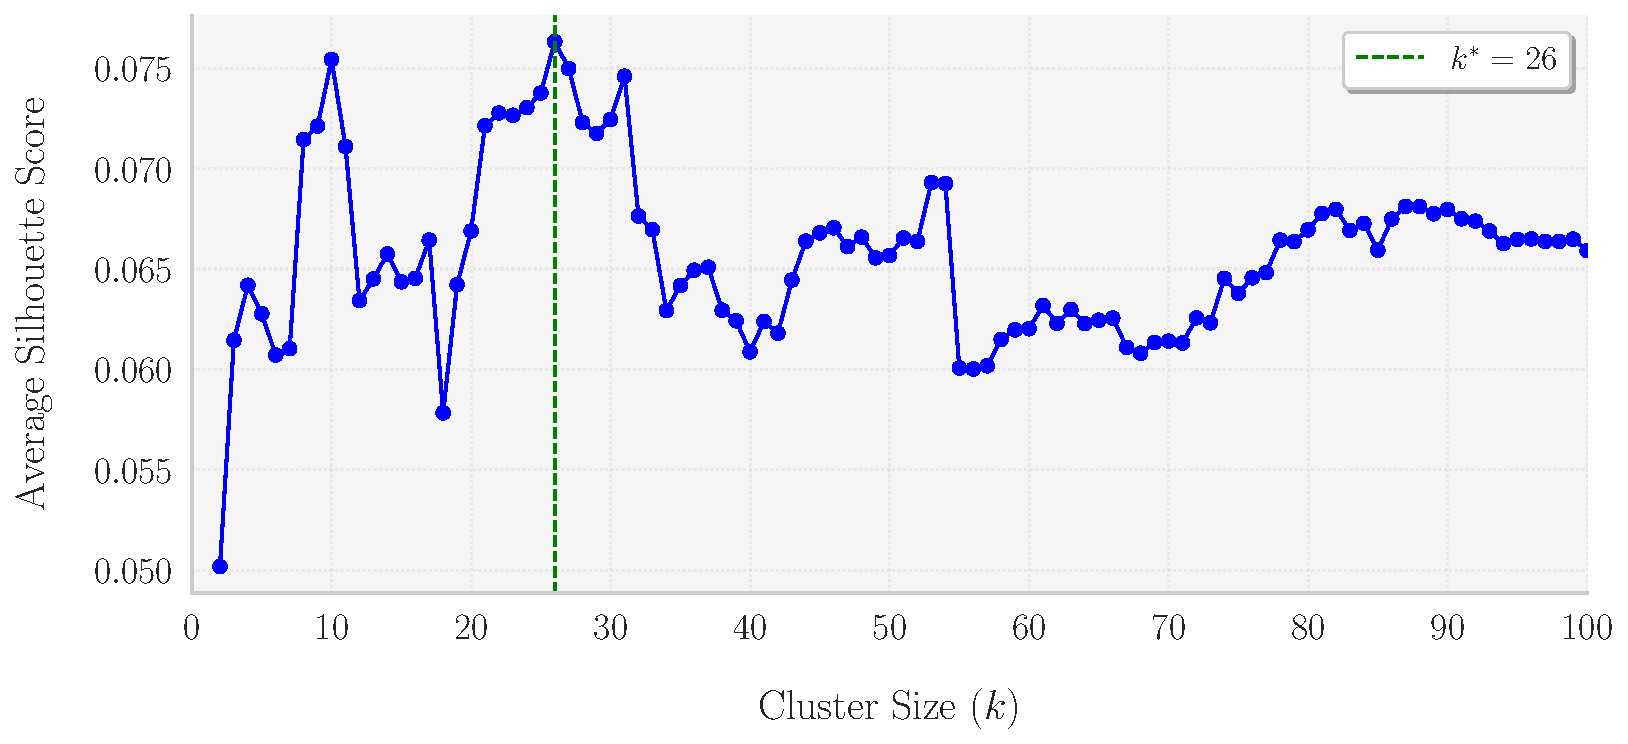
\includegraphics[scale=0.65]{/Users/jesusvillotamiranda/Library/CloudStorage/OneDrive-UniversidaddeLaRioja/CEMFI/__MSc__/__Second_year__/6th_Term/MasterThesis/__Output/KMeans_Clustering_Silhouette_Score.pdf}
\subcaption*{\textit{Note: This plot shows the average silhouette scores computed on $\D^{tr}$ over a grid of possible cluster sizes $\mbf k=\{2,...,100\}$. The maximizer $k^*=26$ is highlighted with a vertical dashed green line.}}
\label{fig:silhouette_score}
\end{figure}
%----------------------------------------------------




\mx
Given the optimal number of clusters $k^*$, we fit the KMeans algorithm on the training embeddings 
$\{\mbf e^i \mid i\in\D^{tr}\}$
%$\{ \mathbf{e}^1, \mathbf{e}^2, \ldots, \mathbf{e}^{N_{tr}} \}$
 to obtain the centroids $\{ \mathbf{c}^{tr}_1, \mathbf{c}^{tr}_2, \ldots, \mathbf{c}^{tr}_{k^*} \}$. Following \cref{alg:KMeans} (detailed in section A1 of the Appendix):
$$
\{ \mathbf{c}^{tr}_1, \mathbf{c}^{tr}_2, \ldots, \mathbf{c}^{tr}_{k^*} \} = \text{KMeans} ( \{ \mathbf{e}^1, \mathbf{e}^2, \ldots, \mathbf{e}^{N_{tr}} \}, k^* )
~.
$$

We then find the cluster associated to each embedding $\mathbf{e}^i$ in the validation set 
$\{\mbf e^i \mid i\in\D^{val}\}$ according to the centroids resulting from clustering the training data $\{\mbf c_1^{tr},..., \mbf c_{k^*}^{tr}\}$.
%$\{ \mathbf{e}^{N_{tr}+1}, \mathbf{e}^{N_{tr}+2}, \ldots, \mathbf{e}^{N_{tr}+N_{val}} \}$ to the nearest centroid $\mathbf{c}_g$. 
This allows us to obtain the clustering of the news articles in the validation sample
$$
\D_g^{val} = 
\3{ 
i\in \D^{val} 
\c g = \arg \min_{\ell\in\G} \|\mathbf{e}^i - \mathbf{c}^{tr}_{\ell}\|_{2}^2
}
\quad 
\forall g\in\G
.
$$

Similarly, by assigning each embedding $\mathbf{e}^i\in \{\mbf e^i \mid i\in\D^{test}\}$
 to the nearest centroid $\mathbf{c}^{tr}_g$, we obtain the clusters in the test set
$$
\D_g^{test} = 
\3{ 
i\in \D^{test}
\c g = \arg \min_{\ell\in\G} \|\mathbf{e}^i - \mathbf{c}^{tr}_{\ell}\|_{2}^2 
}
\quad 
\forall g\in\G
.
$$
%----------------------------------------------------

%
%%----------------------------------------------------
%\begin{figure}[H]
%  \centering
%  \caption{Distribution of articles through KMeans clusters}
%  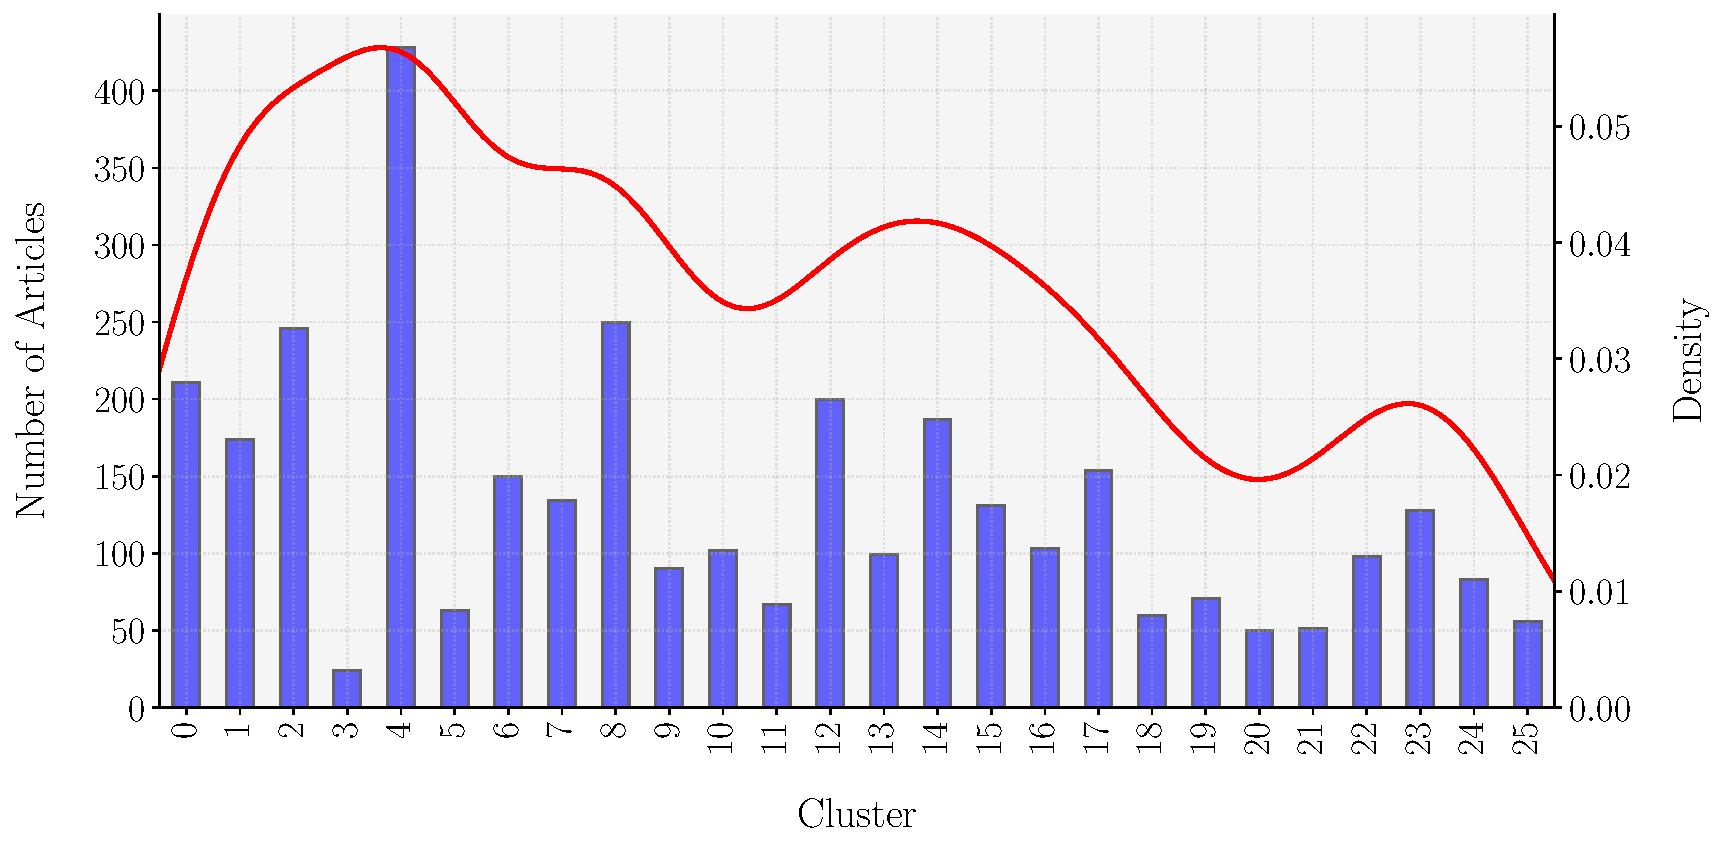
\includegraphics[scale=0.6]{/Users/jesusvillotamiranda/Library/CloudStorage/OneDrive-UniversidaddeLaRioja/CEMFI/__MSc__/__Second_year__/6th_Term/MasterThesis/__Output/KMeans_Cluster_Distribution.pdf}
%%  \caption{}
%\end{figure}
%%----------------------------------------------------
%
%
%%----------------------------------------------------
%\begin{figure}[h!]
%    \centering
%%    \caption{Distribution of articles through KMeans clusters across data splits}
%    \begin{subfigure}[b]{0.32\textwidth}
%        \centering
%        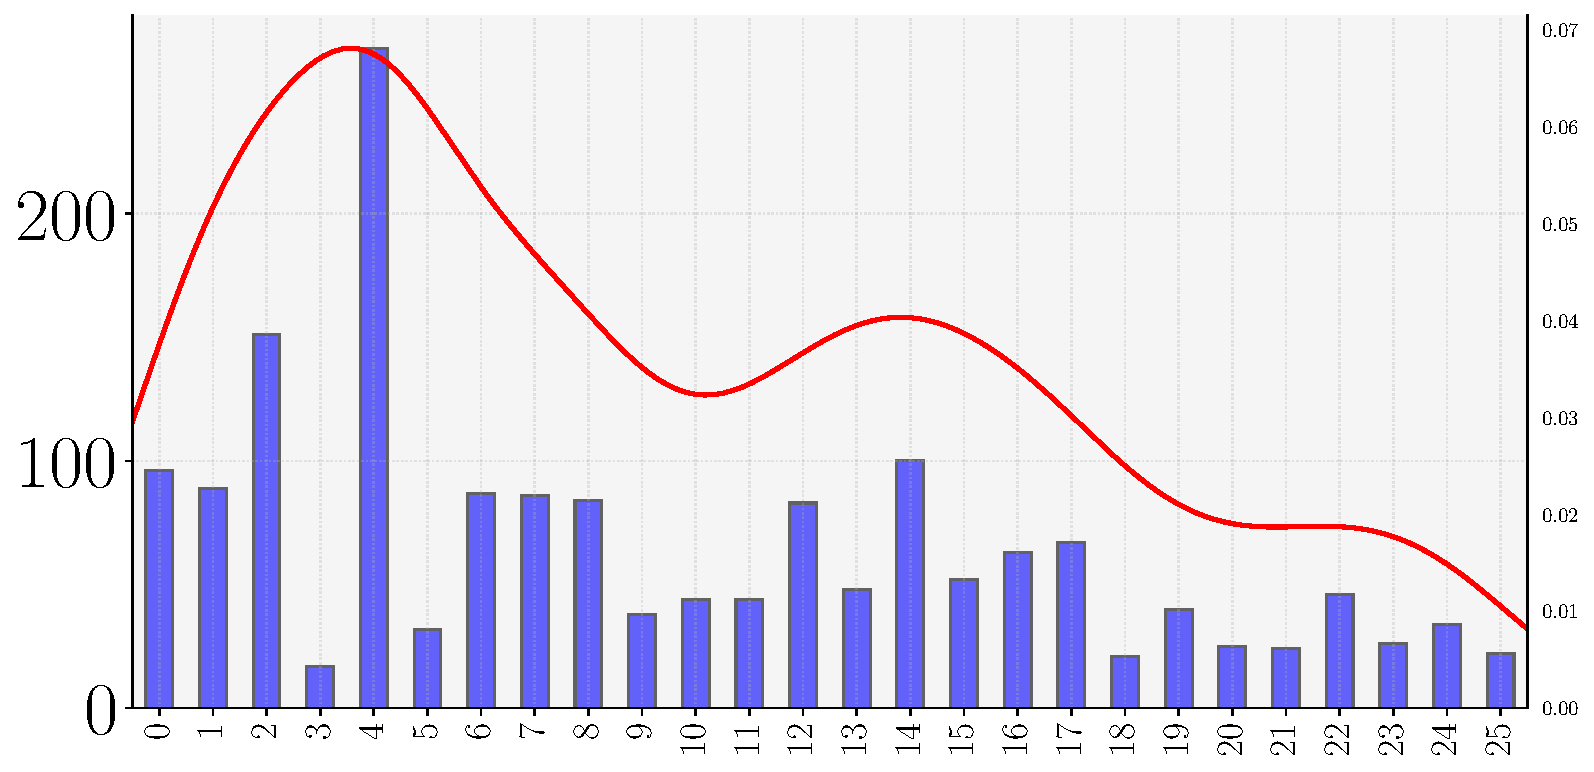
\includegraphics[width=\textwidth]{/Users/jesusvillotamiranda/Library/CloudStorage/OneDrive-UniversidaddeLaRioja/CEMFI/__MSc__/__Second_year__/6th_Term/MasterThesis/__Output/KMeans_Cluster_Distribution_Train.pdf}
%        \caption{Training data ($D^{tr}$)}
%        \label{fig:plot1}
%    \end{subfigure}
%    \begin{subfigure}[b]{0.32\textwidth}
%        \centering
%        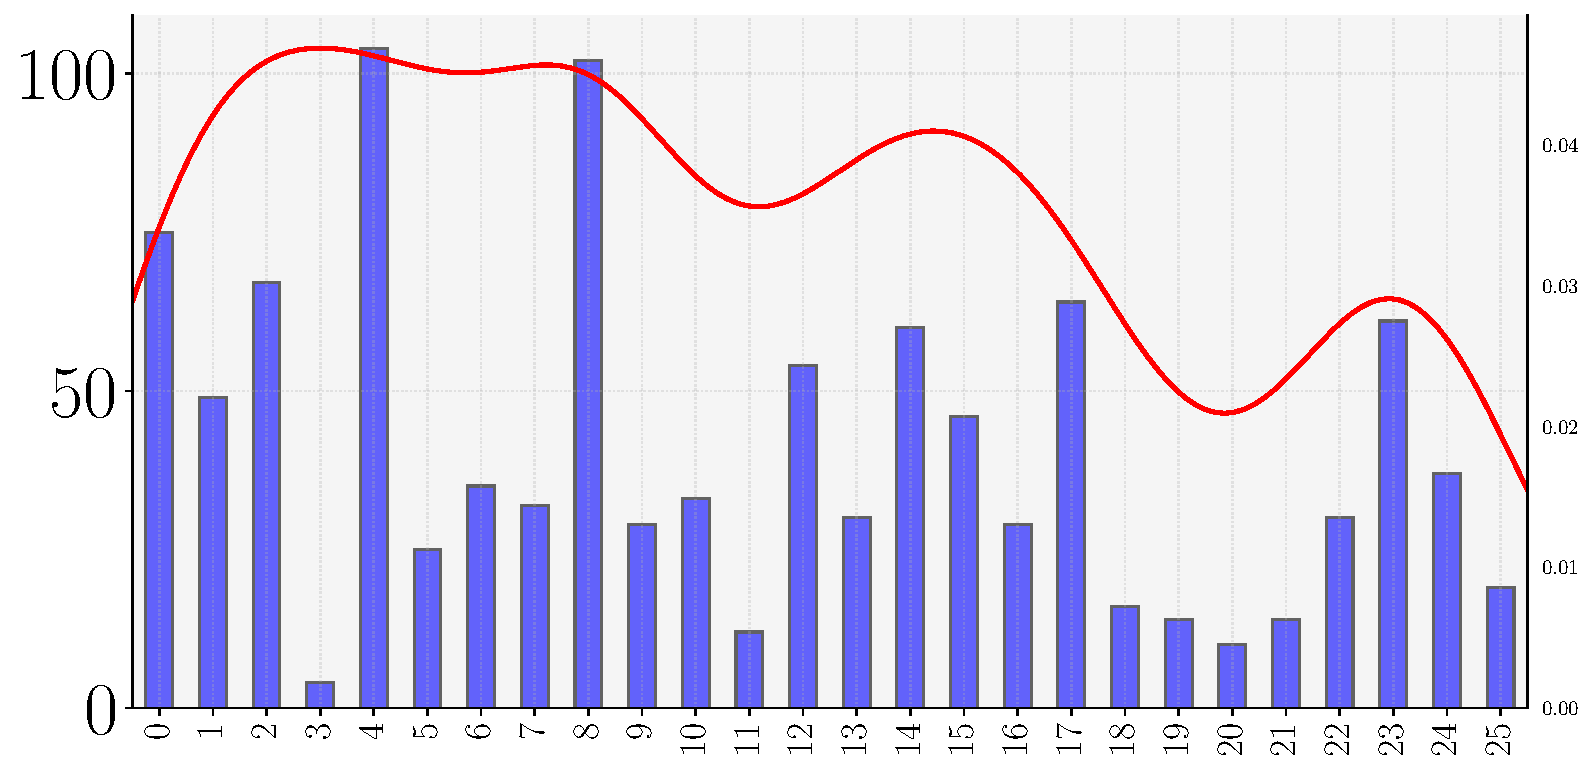
\includegraphics[width=\textwidth]{/Users/jesusvillotamiranda/Library/CloudStorage/OneDrive-UniversidaddeLaRioja/CEMFI/__MSc__/__Second_year__/6th_Term/MasterThesis/__Output/KMeans_Cluster_Distribution_Validation.pdf}
%        \caption{Validation data ($D^{val}$)}
%        \label{fig:plot2}
%    \end{subfigure}
%    \begin{subfigure}[b]{0.32\textwidth}
%        \centering
%        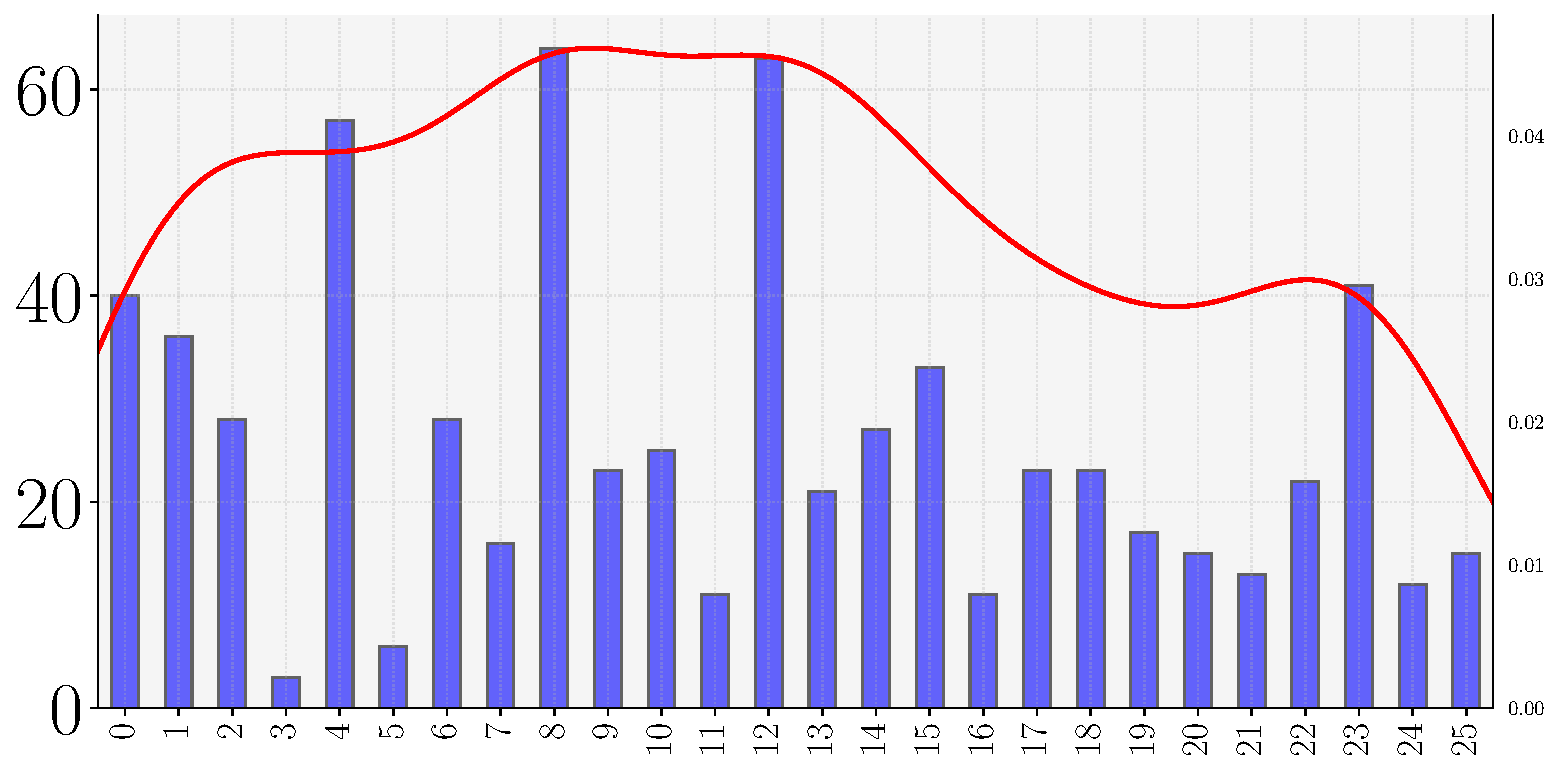
\includegraphics[width=\textwidth]{/Users/jesusvillotamiranda/Library/CloudStorage/OneDrive-UniversidaddeLaRioja/CEMFI/__MSc__/__Second_year__/6th_Term/MasterThesis/__Output/KMeans_Cluster_Distribution_Test.pdf}
%        \caption{Test data ($D^{test}$)}
%        \label{fig:plot3}
%    \end{subfigure}
%    \label{fig:three_plots}
%\end{figure}
%%----------------------------------------------------

%----------------------------------------------------
\inserthere{fig:combined_plots}
\begin{figure}[H]
    \centering
    \caption{Distribution of articles through KMeans clusters}
    
    % Upper plot
    \begin{subfigure}[b]{\textwidth}
        \caption{All data ($\mathcal D$)}
        \centering
        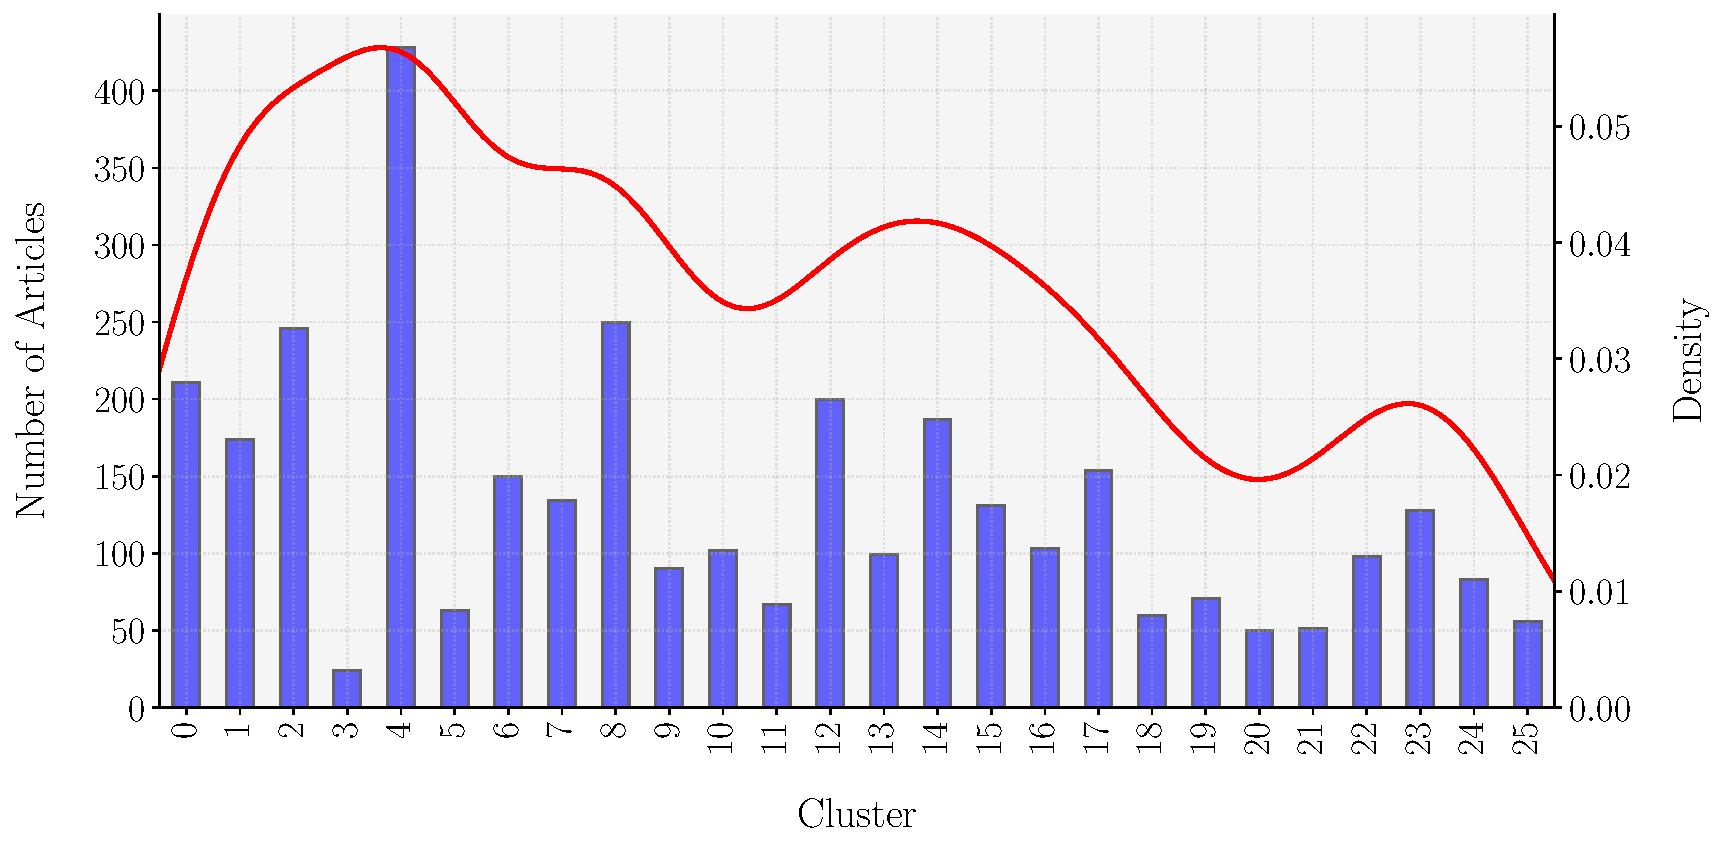
\includegraphics[scale=0.45]{/Users/jesusvillotamiranda/Library/CloudStorage/OneDrive-UniversidaddeLaRioja/CEMFI/__MSc__/__Second_year__/6th_Term/MasterThesis/__Output/KMeans_Cluster_Distribution.pdf}
        \label{fig:all_data}
    \end{subfigure}

    % Lower plots
    \begin{subfigure}[b]{0.32\textwidth}
        \caption{Training data ($\D^{tr}$)}
        \centering
        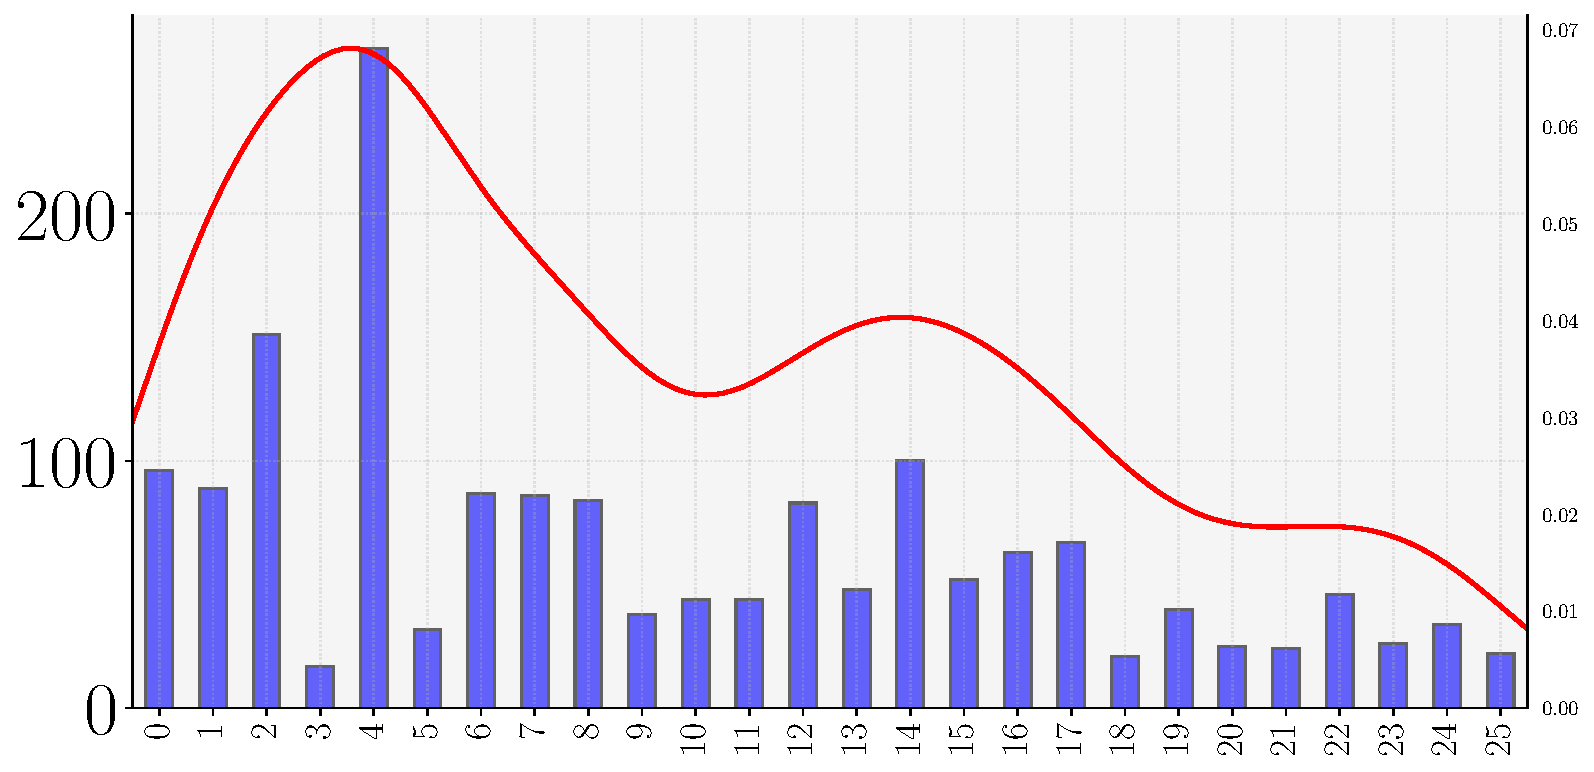
\includegraphics[width=\textwidth]{/Users/jesusvillotamiranda/Library/CloudStorage/OneDrive-UniversidaddeLaRioja/CEMFI/__MSc__/__Second_year__/6th_Term/MasterThesis/__Output/KMeans_Cluster_Distribution_Train.pdf}
        \label{fig:train_data}
    \end{subfigure}
    \begin{subfigure}[b]{0.32\textwidth}
        \caption{Validation data ($\D^{val}$)}
        \centering
        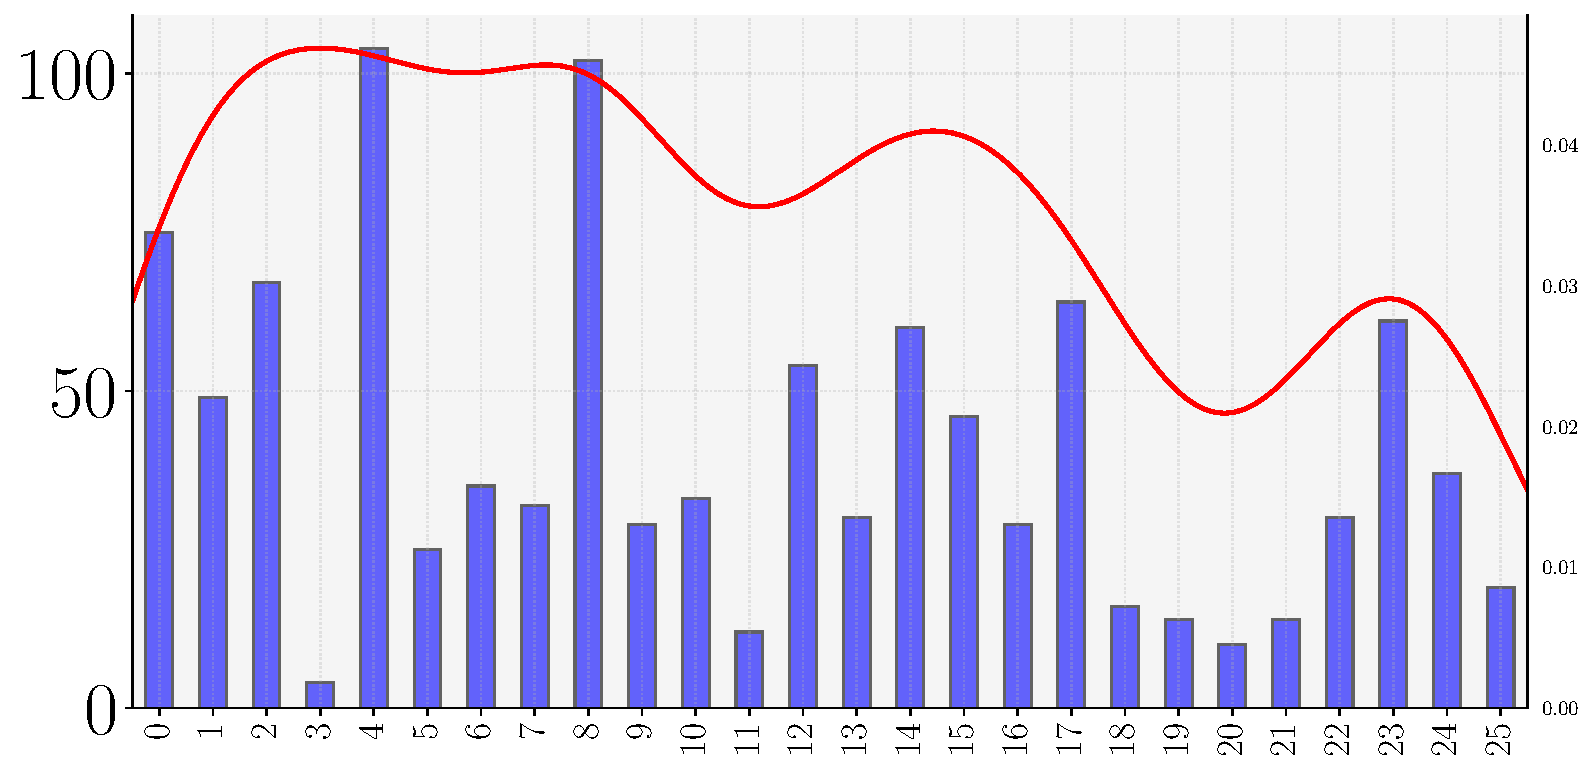
\includegraphics[width=\textwidth]{/Users/jesusvillotamiranda/Library/CloudStorage/OneDrive-UniversidaddeLaRioja/CEMFI/__MSc__/__Second_year__/6th_Term/MasterThesis/__Output/KMeans_Cluster_Distribution_Validation.pdf}
        \label{fig:val_data}
    \end{subfigure}
    \begin{subfigure}[b]{0.32\textwidth}
        \caption{Test data ($\D^{test}$)}
        \centering
        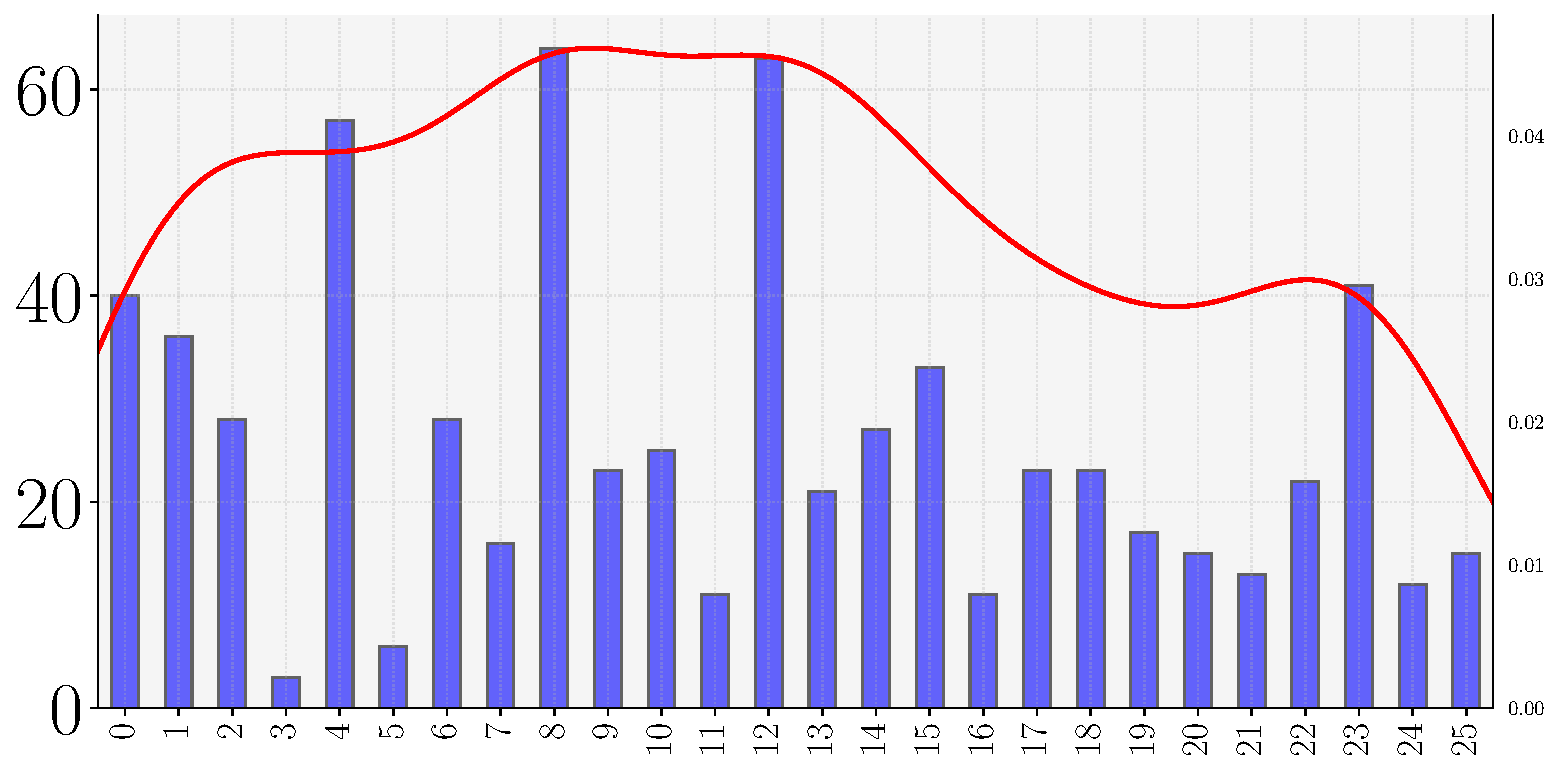
\includegraphics[width=\textwidth]{/Users/jesusvillotamiranda/Library/CloudStorage/OneDrive-UniversidaddeLaRioja/CEMFI/__MSc__/__Second_year__/6th_Term/MasterThesis/__Output/KMeans_Cluster_Distribution_Test.pdf}
        \label{fig:test_data}
    \end{subfigure}
    \label{fig:combined_plots}
\subcaption*{\textit{Note: The upper plot shows the distribution of all the articles $i\in \mathcal D$ through the KMeans clusters, while the lower plots show the distributions for the training ($\D^{tr}$), validation ($\D^{val}$), and test ($\D^{test}$) articles respectively.}}
\end{figure}
%----------------------------------------------------

As we can see, the distribution of articles in the whole sample ($\D$) is fairly homogenous across the 26 clusters, with each cluster containing between 50 and 250 articles on average. The notable exceptions are cluster 3, which contains only 24 articles, and cluster 4, which concentrates 428 articles. However, the distribution profile is not consistent over data splits, which indicates that this classification procedure is unstable over time.

\mx 
Although not directly interpretable, by looking at the articles pooled in a certain cluster, we can provide some intuition of what it represents. In most cases, each cluster contains articles involving a firm or set of firms in the same sector. For example, cluster 3 pools articles about Telef�nica and Cellnex (telecoms), cluster 4 contains articles about CaixaBank, cluster 9 concentrates articles about Repsol, cluster 12 about Iberdrola, cluster 15 gathers articles on Infrastructure (led by ACS and Acciona) and so on.

\mx 
However, there are some exceptions to this general rule, for example, cluster 0 is a \qquote{miscellanous} cluster:
% with no clear pattern: 
 it covers articles about different firms with no apparent relation between them. Another example is cluster 1, which pools articles related to the quarterly or semiannual publication of results by different firms. In \cref{tab:KMeans_Articles_3_English} of the Appendix we provide a sample of 3 articles for each cluster and propose a name for each one based on the articles they pool.


%Even though the interpretation of the clusters is not always clear, we can try to provide a general topic to each of them based on the type of articles that they contain.


%
%\red{Explain what each cluster means and provide examples of articles in each of the clusters}
%
%
%Despite a few exceptions, the distribution of articles by cluster is fairly homogeneous, with each cluster containg between 100 and 250 articles on average. The notable exceptions are clusters 3, with only \red{20?: CHECK} articles, and cluster 4, with over 400 articles. 
%
%




%%%%%%%%%%%%%%%%%%%%%%%%%%%%%%%%%%%%%%%%%%%%%%%%%%%%%
%%%%%%%%%%%	   DELETE BELOW   %%%%%%%%%%%%%%%%%%%%%%%
%%%%%%%%%%%%%%%%%%%%%%%%%%%%%%%%%%%%%%%%%%%%%%%%%%%%%

%\subsection{Notation for trading days}
%To facilitate the understanding and implementation of our trading strategy, we introduce a clear and systematic notation for handling trading days. We define 
%%the ordered set trading days as 
%$\tilde{\mathfrak{d}}=\3{\tilde{\mathfrak{d}}_1, \tilde{\mathfrak{d}}_2, \ldots}$, representing an ordered sequence of trading days. To map a specific trading day $\tilde{d} \in \tilde{\mathfrak{d}}$ to its position within this sequence, we define the Index function $\mathbb{I}_{\tilde{\mathfrak{d}}}: \tilde{d} \in \tilde{\mathfrak{d}} \longrightarrow \{1, 2, \ldots, |\tilde{\mathfrak{d}}|\}$. For any given trading day $\tilde{d} = \tilde{d}_k \in \tilde{\mathfrak{d}}$, the Index function $\mathbb{I}_{\tilde{\mathfrak{d}}}(\tilde{d})$ returns its position $k$. Conversely, the function $\mathbb{D}_{\tilde{\mathfrak{d}}}(k)$ retrieves the trading day corresponding to a given index $k$, ensuring the ordered structure is maintained. Additionally, for any date $d$ not in $\tilde{\mathfrak{d}}$, the operator $\Lambda(d)$ returns the next closest trading day within $\tilde{\mathfrak{d}}$. This systematic notation is crucial for accurately defining trading windows, such as the market model window $[\mathbb{D}_{\tilde{\mathfrak{d}}}(\mathbb{I}_{\tilde{\mathfrak{d}}}(\tilde{d}_0^i) - \widetilde{w}_b - \widetilde{w}_m), \mathbb{D}_{\tilde{\mathfrak{d}}}(\mathbb{I}_{\tilde{\mathfrak{d}}}(\tilde{d}_0^i) - \widetilde{w}_b)]$, ensuring both start and end points are valid trading days. This notation aids in defining the trading rule $T R_{L, \theta}$ and the portfolio $\mathcal{P}$ precisely, enhancing the robustness and clarity of our strategy's implementation.
%
%
%\textbf{Market Model Window Definition}
%
%For each unique pair $(i, j) \in \mathcal{B}$, we fit a market model on some window
%$\mathcal{M}:=$
% before the news publication date $\tilde{d}_0^i$. The market model window is defined using the above notation to ensure start and end points are both trading days:
%$$
%r_{\tilde{d}}^j = \alpha^{(i, j)} + \beta^{(i, j)} r_{\tilde{d}}^M + \epsilon_{\tilde{d}}^{(i, j)} \quad \text{for } \tilde{d} \in 
%\left[ 
%\mathbb{D}_{\tilde{\mathfrak{d}}} \left( \mathbb{I}_{\tilde{\mathfrak{d}}} (\tilde{d}_0^i) - \widetilde{w}_b - \widetilde{w}_m \right), \mathbb{D}_{\tilde{\mathfrak{d}}} 
%\left( \mathbb{I}_{\tilde{\mathfrak{d}}} (\tilde{d}_0^i) - \widetilde{w}_b 
%\right) 
%\right],
%$$
%where $\widetilde{w}_b$ denotes the buffer window (10 trading days) and $\widetilde{w}_m$ denotes the market model window (100 trading days).
%
%\textbf{Trading Rule and Portfolio Definition}
%
%For a given selection of clusters $\mathcal{G}_\theta^{+}$ and $\mathcal{G}_\theta^{-}$, we launch trades with a holding period of $L$ trading days. The trading rule $T R_{L, \theta}\langle(i, j), \tilde{d}\rangle$ for a pair $(i, j) \in \mathcal{B}$ at trading day $\tilde{d}$ is defined as follows.
%
%In this context, a portfolio is a collection of positions taken in firm's stocks according to $T R_{L, \theta}\langle(i, j), \tilde{d}\rangle$. In other words, it is the set of all $\langle(i, j), \tilde{d}\rangle$ for which a trade is executed:
%\[
%\mathcal{P}: = \3{\langle(i, j), \tilde{d}\rangle \mid (i, j) \in \mathcal{B} \wedge \tilde{d} \in \tilde{\mathfrak{d}} \wedge T R_{L, \theta}\langle(i, j), \tilde{d}\rangle \neq 0 }.
%\]
%
%The return of the portfolio on trading date $\tilde{d}$, denoted as $r_{\tilde{d}}^{\mathcal{P}}$, is the average return of the individual positions:
%\[
%r_{\tilde{d}}^{\mathcal{P}} = \frac{1}{|\mathcal{P}_{\tilde{d}}|} \sum_{\langle(i, j), \tilde{d}\rangle \in \mathcal{P}_{\tilde{d}}} AR_{\tilde{d}}^{(i, j)},
%\]
%where $\mathcal{P}_{\tilde{d}} = \3{\langle(i, j), \tilde{d}\rangle \in \mathcal{P} \mid \tilde{d} - L + 1 \leq \tilde{d} \leq \tilde{d} }$ represents the set of open positions on trading day $\tilde{d}$.

%%%%%%%%%%%%%%%%%%%%%%%%%%%%%%%%%%%%%%%%%%%%%%%%%%%%%
%%%%%%%%%%%	   DELETE ABOVE   %%%%%%%%%%%%%%%%%%%%%%%
%%%%%%%%%%%%%%%%%%%%%%%%%%%%%%%%%%%%%%%%%%%%%%%%%%%%%




%----------------------------------------------------
\subsection{Beta-neutral positions on every $(i,j)\in\mathcal B$}
Since we are interested in the individual effect of an article $i\in\D$ in each of the affected firms $j\in\F^i$, we define the set
$
\mathcal{B}:=\3{(i,j) \mid i\in \D ~\wedge~j\in \F^i }
$, where $\abs{\mathcal{B}}=3410>\abs{\D}=2613$. 
We then fit a market model to each unique pair $(i,j)\in \mathcal{B}$
%consisting of a firm $j\in\F^i$ affected by article $i$ 
on some window of time $\mathcal{M}^i\subset \tilde{\mathfrak{d}}$ before the effective treatment day: 
\footnote{To rigorously define $\mathcal M^i$, we need to work with the index and inverse index functions. 
\begin{itemize}
  \item \textbf{Index Function}. 
Given a finite ordered set $\mathcal{Z}=\left\{z_1, z_2, \ldots, z_n\right\}$, the index function 
$\mathbb{I}_{\mathcal{Z}}: \mathcal{Z} \rightarrow\{1,2, \ldots,|\mathcal{Z}|\}$
%$\mathbb{I}_{\mathcal{Z}}(z)$
 maps an element $z\in\Z$ to its position in the ordered set $\mathcal{Z}$. Formally:
$
\mathbb{I}_{\mathcal{Z}}(z_{\ell})=\ell 
%\quad \text { if and only if } \quad z=z_{\ell} 
~ \text { for } ~ \ell \in\{1,2, \ldots,|\mathcal{Z}|\}
.
$
%where $z_{\ell}$ denotes the ${\ell}$-th element of the ordered set $\mathcal{Z}$.

\item \textbf{Inverse Index Function}. 
The inverse index function 
$\mathbb{I}_{\mathcal{Z}}^{-1}:\{1,2, \ldots,|\mathcal{Z}|\} \rightarrow \mathcal{Z}$
%$\mathbb{I}_{\mathcal{Z}}^{-1}({\ell})$
 retrieves the element $z \in \mathcal{Z}$ corresponding to a given index ${\ell}$.
Formally:
$
\mathbb{I}_{\mathcal{Z}}^{-1}({\ell})=z_{\ell} ~\text { for } ~{\ell} \in\{1,2, \ldots,|\mathcal{Z}|\}
.$
\end{itemize}
For the market model window, we use $\mathbb{I}_{\tilde{\mathfrak{d}}}$ and $\mathbb{I}^{-1}_{\tilde{\mathfrak{d}}} $ applied to the set of trading days $\tilde{\mathfrak d}$. Namely:
$$
\mathcal{M}^i := 
\3{
d\in \tilde{\mathfrak{d}}
\c 
\mathbb{I}^{-1}_{\tilde{\mathfrak{d}}} 
\1{
\mathbb{I}_{\tilde{\mathfrak{d}}} (\tilde{d}_0^i) - {w}_b - {w}_m 
}
\leq d \leq 
\mathbb{I}^{-1}_{\tilde{\mathfrak{d}}} 
\1{ 
\mathbb{I}_{\tilde{\mathfrak{d}}} (\tilde{d}_0^i) - {w}_b 
}
}
,
$$
with a buffer of ${w}_b=10$ trading days before the effective treatment date, and a market model window length of ${w}_m=100$ trading days.



}
%----------------------------------------------------
$$
r_{d}^{j} = \alpha^{(i,j)} + \beta^{(i,j)} r_{d}^M + \epsilon_{ d}^{(i,j)} 
\qquad  
%\t{for}
%~
%\qquad
\forall d \in \mathcal{M}^i
,
$$
%\begin{align*}
%r_{\tilde d}^{j} = \alpha^{(i,j)} + \beta^{(i,j)} r_{\tilde d}^M + \epsilon_{\tilde d}^{(i,j)} 
%\qquad  
%\t{for}
%~
%%\qquad
%\tilde d \in 
%\5{
%\tilde d_0^i - \widetilde{w}_b - \widetilde{w}_m
%~,~
%\tilde d_0^i - \widetilde{w}_b
%}
%,
%\end{align*}
where 
$r_{d}^{j}$ denotes the return of firm $j$ at trading day $d$ in excess of the risk-free asset, which we take to be the daily euro short-term rate (\texttt{\euro STR}),
and 
$r_{d}^M$ denotes the excess return of the market (IBEX-35).  
%----------------------------------------------------
These returns are obtained from the adjusted close price, which corrects the price evolution for corporate actions such as dividends, stock splits, and new stock issuance.\footnote{
The adjusted close price ensures that the returns reflect the true economic gains or losses for an investor holding the stock. 
%
Formally, the return of firm $j$ between two trading days $d_1, d_2\in \tilde{\mathfrak{d}}$ is computed as:
$
r_{d_1:d_2}^{j} = 
%\frac{
(
p_{d_2}^{j,\text{adj}} - p_{d_1}^{j,\text{adj}}
%}{
)/(
p_{d_1}^{j,\text{adj}}
)
%},
$
where $p_{d}^{j,\text{adj}}$ is the adjusted close price of firm $j$ at trading day $d$.
}
%----------------------------------------------------

\mx 
%----------------------------------------------------
The notation overload in the regression coefficients $(\alpha^{(i,j)},\beta^{(i,j)})$ emphasizes the fact that $\alpha$ and $\beta$ are specific to each pair $(i,j)\in\mathcal B$ since the market model is computed for each firm $j\in\F_{\t{IBEX-35}}$ on some specific window of time $\mathcal{M}^i$, which is particular to each article $i\in\D$.
%----------------------------------------------------

\mx 
The reason why we fit a market model to each $(i,j)\in\mathcal B$ is to then apply a market-neutral strategy as in \cite{chan2003stock} and \cite{jiang2021pervasive}. This is an investment approach designed to minimize or eliminate exposure to overall market movements, isolating the performance of a specific firm. 
%The primary goal is to achieve positive returns regardless of the market's direction (up or down). 
In particular, we employ a beta-neutral strategy by buying one unit of firm $j$'s stock and shorting $\beta^{(i,j)}$ units of the market index (i.e.: an ETF replicating the IBEX-35). 

%where $\beta^{(i,j)}$ is the sensitivity of the firm's stock to the market. 

% This approach allows us to isolate the impact of news articles on individual stock performance without the confounding influence of market-wide movements.

%This approach neutralizes the impact of broad market movements, allowing us to focus on the abnormal returns generated by specific news events. 
%This beta-neutral strategy isolate the impact of news articles on individual stock performance without the confounding influence of market-wide movements.


%\mx 
%Based on the estimates $( \alpha^{(i,j)},  \beta^{(i,j)})$, we apply a market-neutral strategy, which is an investment approach designed to minimize or eliminate exposure to overall market movements, isolating the performance of firm $j$. The primary goal is to achieve positive returns regardless of the market's direction (up or down). In this strategy, long positions are taken in firms expected to outperform the market, and short positions are taken in firms expected to underperform. 

%The beta-neutral aspect involves adjusting the portfolio so that the weighted average beta is zero, meaning the portfolio's value should not be affected by market movements. This reduces market risk and focuses on the performance of selected securities. By employing a beta-neutral strategy in this thesis, we aim to isolate the impact of news articles on individual stock performance without the confounding influence of market-wide movements.
%----------------------------------------------------
\mx
This hedged position harvests the idiosyncratic returns from the market model and it only makes sense when firm $j$'s returns are expected to outperform or underperform the market.\footnote{
For expected underperformance of firm $j$, reverse the beta neutral positions: 
sell one unit of firm $j$ and buy $\beta^{(i,j)}$ units of the market index. However, note that this will be handled later by a Trading Rule $(TR)$.
%Note that in the case of expected underperformance of firm $j$, the beta neutral positions should be reversed: sell one unit of firm $j$ and buy $\beta^{(i,j)}$ units of the market index. But for now, there is no need to be concerned with this: the ultimate construction of the positions will be managed by the later introduced Trading Rule $(TR)$.
\mx 
}
The position delivers abnormal returns $AR^{(i,j)}_{d}$ at some trading day $d\geq \tilde{d}_0^i$ given by
%
%Based on the estimates $( \alpha^{(i,j)},  \beta^{(i,j)})$, we compute the returns of a position that buys firm $j$'s stock and sells $ \beta^{(i,j)}$ times the market (by entering into a short position in an ETF that replicates the IBEX-35 Index). This hedged position delivers abnormal returns at trading date $\tilde d$ given by
\begin{align*}
r_{d}^j -  \beta^{(i,j)} r_{d}^M = \alpha^{(i,j)} + \epsilon_{d}^{(i,j)} =: AR^{(i,j)}_{d}
.
\end{align*}
%----------------------------------------------------
The position is taken at the effective treatment date $\tilde d_0^i$ and is maintained over a holding window $\mathcal H^i \subset \tilde{\mathfrak{d}}$ consisting of $L\in\mathbb{N}$ trading days after $\tilde d_0^i$, where $L$ is set to 4 trading days.\footnote{  
The holding period of the position is defined as 
$
\mathcal H^i:=
\3{
d \in \tilde{\mathfrak{d}}
\c 
\tilde{d}_0^i
\leq d \leq 
\mathbb{I}^{-1}_{\tilde{\mathfrak{d}}}\1{\mathbb{I}_{\tilde{\mathfrak{d}}}(\tilde d_0^i)+L}}
%\mathbb{D}_{\tilde{\mathfrak{d}}}\1{\mathbb{I}_{\tilde{\mathfrak{d}}}(\tilde d_0^i)+L}}
$}
%----------------------------------------------------
The justification for this choice of $L$ is made in section A.2 of the Appendix. 

%----------------------------------------------------
\mx 

After having held the beta-neutral position over the holding period $\mathcal H^i$, we obtain a time series of abnormal returns $\{AR_{d}^{(i,j)}\}_{d\in\mathcal H^i}$ from where we can obtain the usual performance metrics. First, the average daily log returns are obtained as
$$
\mu^{(i,j)} = \frac{1}{{{L}}+1} 
%\sum_{d=\tilde d_0^i }^{\tilde d_0^i + {{L}}} 
\sum_{d\in \mathcal H^i}
\ln\4{1+AR_d^{(i,j)}}
~,
$$
%$
%\mu_{{{L}}}^{(i,j)}
%=
%\1{1+CAR_{{{L}}}^{(i,j)}}^{1/({{L}}+1)}-1,
%$
Then, the standard deviation is given by
$$
\sigma^{(i,j)}
=
\sqrt{
\frac{1}{{{L}}}
\sum_{d\in \mathcal H^i}
%\sum_{d=\tilde d_0^i }^{\tilde d_0^i + {{L}}} 
[
\ln(1+AR_d^{(i,j)}) - \mu^{(i,j)}
]
^2}
~.
$$

\mx 
And finally, the annualized Sharpe Ratio can be obtained by scaling the daily Sharpe Ratio by the square root of ${252}$, which are the typical number of trading days in a year according to the Spanish calendar. 
%.  $\sqrt{|\tilde{\mathfrak d}_y|}$
%$
%\sigma_{{{L}}}^{(i,j)}
%= \sqrt{\frac{1}{{{L}}} \sum_{d=\tilde d_0^i}^{\tilde d_0^i + {{L}}} 
%\1{ AR_d^{(i,j)} -\mu_{{{L}}}^{(i,j)} }^2}
%$
$$
SR^{(i,j)} =
\sqrt{252}~
\frac{
\mu^{(i,j)}
}{
\sigma^{(i,j)}
}
%\sqrt{|\tilde{\mathfrak d}_y|}
~.
$$
%%%%%%%%%%%%%%%%%%%%%%%%%%%%%%%%%%%%%%%%%%%%%%%%%%%%%
\subsection{Optimal Cluster Selection}
%%%%%%%%%%%%%%%%%%%%%%%%%%%%%%%%%%%%%%%%%%%%%%%%%%%%%

After taking beta-neutral positions on each pair $(i,j)\in\mathcal B$ and holding them over some window $\mathcal H^i$, we can obtain a measure of how profitable the positions are on average for articles that belong to the same cluster $g\in\mathcal G$. For this purpose, let $\mathcal{B}_g$ denote the set of all article and firm pairs such that the article belongs to some cluster $g\in\mathcal G$. 
$$
\mathcal{B}_g:= \{(i,j) \mid (i,j)\in\mathcal{B} ~\wedge~ i \in \D_g \}
.
$$
The average Sharpe Ratio associated to each cluster is
$$
\overline{S R}_g=\frac{1}{\left|\mathcal{B}_g\right|} \sum_{(i,j) \in \mathcal{B}_g} S R^{(i,j)}
,
$$
and it provides a measure of the performance of the beta-neutral positions in each cluster. 
The distribution of cluster-average Sharpe Ratios across the different clusters is plotted in \cref{fig:KMeans_distr_avg_SR}. In the validation set, they are centered at 0, but we observe some outliers with unusually low and high average $SR$. On the other hand, the distributions in the train and test data are slightly skewed to the right and show no presence of substantial outliers.

%----------------------------------------------------
\inserthere{fig:KMeans_distr_avg_SR}
\begin{figure}[H]
  \centering
  \caption{Distribution  of Cluster-Average Sharpe Ratios $(\overline{SR}_g)$ by Split}
  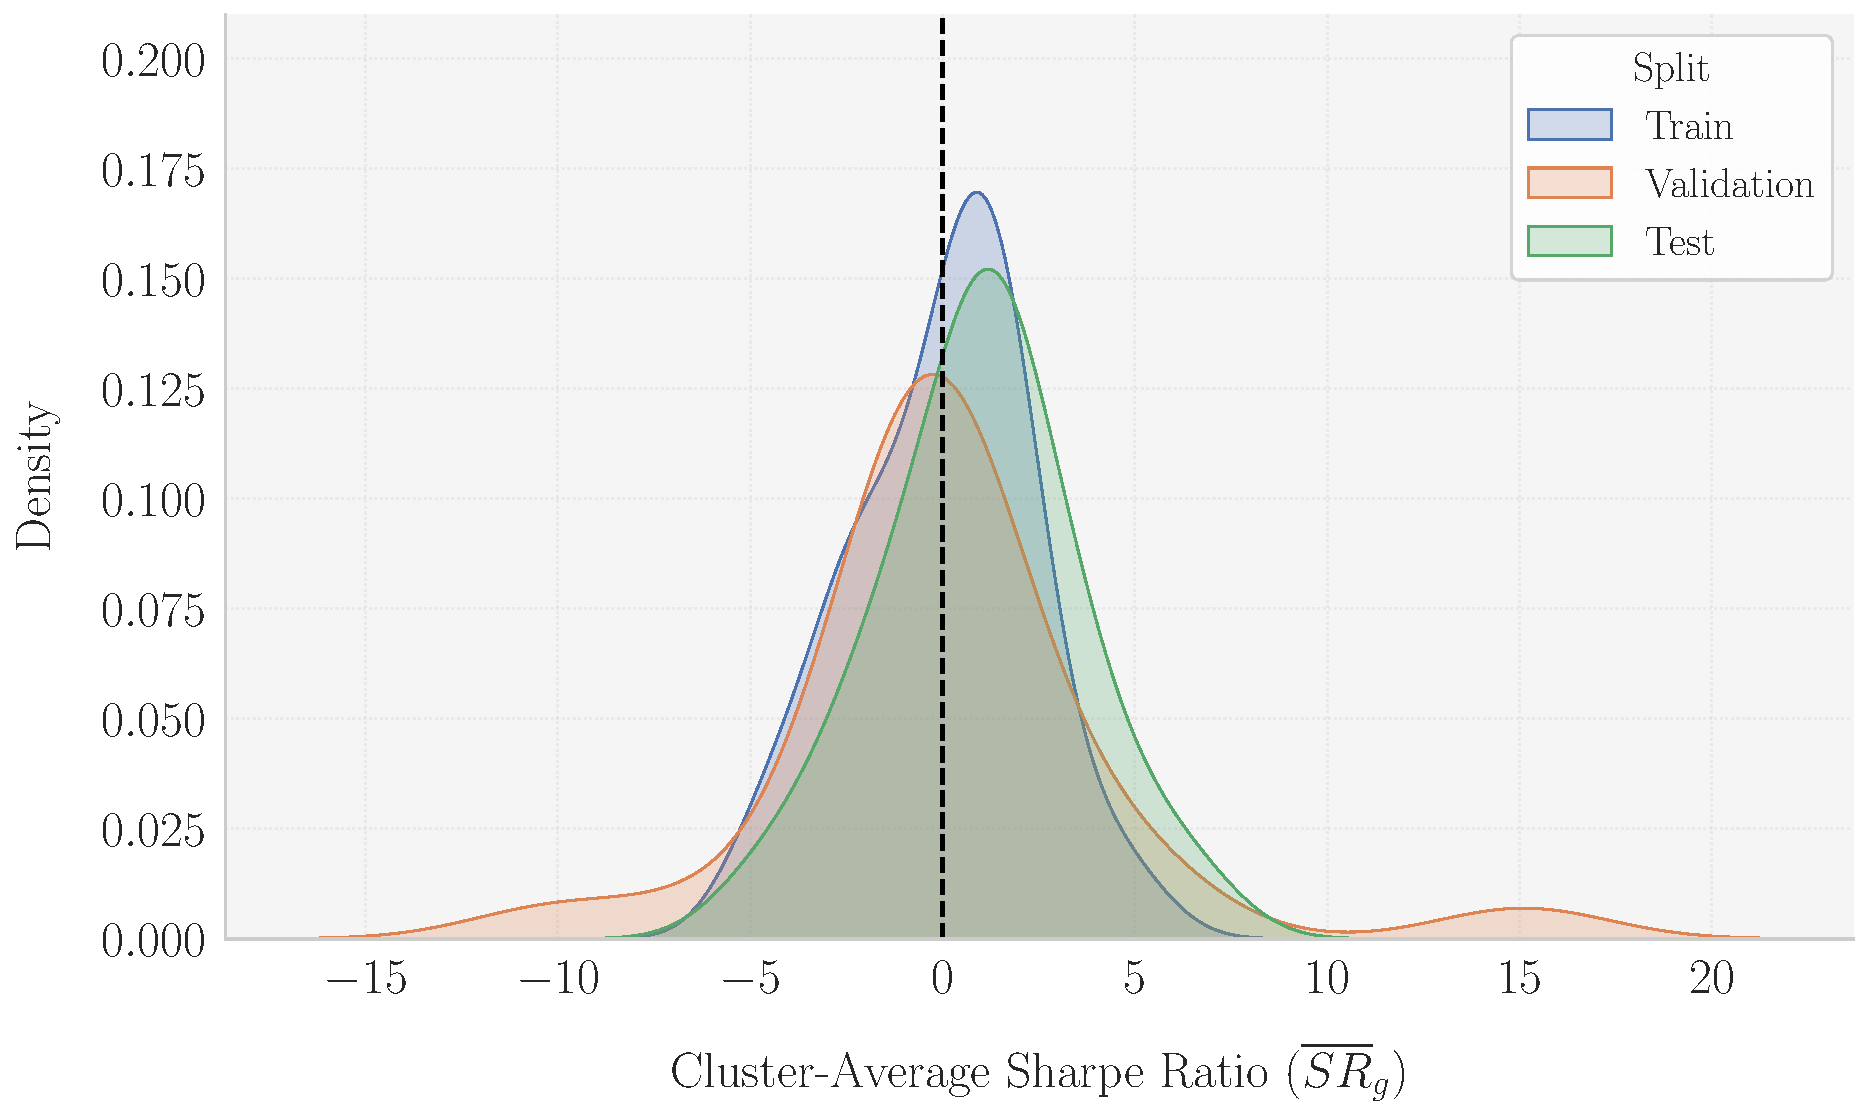
\includegraphics[scale=0.45]{/Users/jesusvillotamiranda/Library/CloudStorage/OneDrive-UniversidaddeLaRioja/CEMFI/__MSc__/__Second_year__/6th_Term/MasterThesis/__Output/KMeans_Cluster-Avg_SR_Distribution.pdf}
\label{fig:KMeans_distr_avg_SR}
\end{figure}
%----------------------------------------------------

\mx
The goal is to now design an algorithm that exploits this information to select the best clusters for the trading strategy. In the remainder of this section, we propose two algorithms. First, an algorithm developed on validation data that will select the clusters maximizing the performance for that split (\qquote{greedy}), and second, an algorithm that will exploit the information from both, training and validation data (higher information set), and whose objective will be to select the most stable clusters among both splits (\qquote{stable}). 


%----------------------------------------------------
%By exploiting the Sharpe Ratios of the beta-neutral positions, we can obtain a simple measure of the profitability of each cluster. In particular, by averaging the annualized Sharpe Ratios of the positions associated to articles that belong to the same cluster. 
%%----------------------------------------------------
%We can then average the annualized Sharpe Ratios of the positions associated to articles that belong to the same cluster. 
%%That is, for each cluster $g$, we compute the average Sharpe Ratio by averaging the Sharpe Ratios of all pairs $(i,j)$ where $i$ belongs to cluster $g$. 
%%--------------- OPTION 1---------------------
%Define $\mathcal{B}_g$ as the set of all pairs $(i,j)\in\mathcal{B}$ such that article $i$ belongs to cluster $g$
%$$
%\mathcal{B}_g:= \{(i,j) \mid (i,j)\in\mathcal{B} ~\wedge~ i \in \D_g \}
%.
%$$
%%--------------- OPTION 2--------------------------- 
%%Formally, let $\mathcal{B}_g$ be the set of all pairs $(i,j)$ such that article $i$ belongs to cluster $g$. 
%%$$\mathcal{B}_g := \{(i,j) \mid  \mbf e^i \in \D_g \}$$
%%----------------------------------------------------
%The average Sharpe Ratio for cluster $g$, denoted as $\overline{S R}_g$, is given by:
%$$
%\overline{S R}_g=\frac{1}{\left|\mathcal{B}_g\right|} \sum_{(i,j) \in \mathcal{B}_g} S R_{{{L}}}^{(i,j)}
%$$


\subsubsection{Greedy Algorithm}

The greedy selection of clusters is done in the validation sample 
$
\mathcal{B}_g^{val}:= \{
%(i,j) \mid 
(i,j)\in\mathcal{B} 
%~\wedge~
 \mid 
  i \in \D_g^{val} \}
~,
$
from where we compute the cluster-average $\overline{S R}_g^{val}$ for each $g\in\G$.
%
%\mx 
%----------------------------------------------------
Define $\mathcal G_{SR^+}^{val}:=\{ g\in \mathcal G \mid \overline{SR}_g^{val} >0\}$ and $\mathcal G_{SR^-}^{val}:=\{ g\in \mathcal G \mid \overline{SR}_g^{val} <0\}$ as the sets of clusters with positive and negative Sharpe Ratios in the validation sample. Obviously, we will be interested in taking long positions when reading an article that is clustered in some $g\in \mathcal G_{SR^+}^{val}$, and short positions in clusters $g\in \mathcal G_{SR^+}^{val}$. 


\mx 
%----------------------------------------------------
However, our trading strategy will not trade every cluster $g\in\G$. Instead, it will select the clusters from $\mathcal G_{SR^+}$ and $\mathcal G_{SR^-}$ that lead the to most profitable trades. 
To identify such clusters, we rank them by their average Sharpe Ratio. Define the ranking function $\mathfrak{R}: \mathcal{G} \to \3{1, \ldots, k^*}$ such that
$$
\mathfrak{R}_g^{val}
=
\sum_{h \in \mathcal{G}} 
\mathbf{1}\1{
\overline{S R}_h^{val} \geq \overline{S R}_g^{val} 
}
$$
where $\mathbf{1}(\cdot)$ is the indicator function which equals 1 if the condition inside is true and 0 otherwise.
%$$
%\overline{SR}^{val}_{{{\varkappa}}_1}\geq  \overline{SR}^{val}_{{{\varkappa}}_2} \geq \ldots \geq \overline{SR}^{val}_{{{\varkappa}}_k}
%$$
%where ${{\varkappa}}_1, {{\varkappa}}_2, \ldots, {{\varkappa}}_{k^*}\in\G$ 
%%denote the indices of the sorted clusters 
%are the clusters sorted in descending order
%such that the subindices $\ell=1,...,k^*$ denote the position of cluster $\varkappa_{\ell}$ in the ranking.

\mx
%----------------------------------------------------
The number of traded clusters on either side (long and short) will be upper-bounded by some hyperparameter of our choice $\theta \in \mathbb{N}$
%$\theta \in \{2 m \mid m \in \mathbb{N}\}$ 
which we set proportional to the optimal number of clusters. Namely, $\theta =\integer{\rho k^*}$ for some $\rho\in(0,1)$, which has been set to $\rho=0.5$ (this choice is justified in section A.2. of the Appendix).
%$\theta\propto k^*$.
%$\theta \in \{2 m \mid m \in \mathbb{N}\}$, which we set proportional to $k^*$.
%$\theta \in\mathbb{E^+}$, where $\mathbb{E}^{+}=\{2 k \mid k \in \mathbb{N}\}$. 
The actual number of traded clusters will not be exactly $\theta$ as there is a natural bound coming from the cardinalities of $\mathcal G_{SR^+}$ and $\mathcal G_{SR^-}$. Hence, the actual number of long and short-traded clusters will be
%$\theta^+$ and $\theta^-$, which are defined as
$
\theta^+ := \min(\theta, ~|\mathcal G_{SR^+}|)
%\quad  
~\t{and}~
%\quad
\theta^- := \min(\theta, ~|\mathcal G_{SR^-}|)
.
$
%
%\mx
%----------------------------------------------------
The set of traded clusters $\mathcal G_{\theta}$ is defined as:
$$
\G_\theta := 
\3{
g \in \mathcal G 
\mid 
1\leq \mathfrak{R}_g^{val} \leq \theta^+
~\vee~ 
k^* -\theta^- < \mathfrak{R}_g^{val} \leq k^*
} 
= 
\G_{\theta}^+ \cup \G_{\theta}^-
~,
$$
where
$
\G_{\theta}^+ := 
\{ g \in\G \mid 
%\varkappa_{\ell} \in \G_{SR^+} \wedge
1\leq \mathfrak{R}_g^{val} \leq \theta^+
\}
$
is the set of long-traded clusters,
%and
$
\G_{\theta}^- := 
\{ g \in\G \mid 
%\varkappa_{\ell} \in \G_{SR^-} \wedge
k^*-\theta^-
< \mathfrak{R}_g^{val} \leq 
k^*
\}
$
is the set of short-traded clusters 
and, clearly, $\abs{\G_{\theta}}=\theta^+ + \theta^- $.\footnote{
Alternatively, we could trade the same number of clusters in the long and short side by defining a unique 
$
\theta^* := \min\1{\theta, |\mathcal G_{SR^+}|, |\mathcal G_{SR^-}| }
%,
$
such that
%In this case, we would have
$
\G_\theta := 
\3{
g \in \mathcal G 
\mid 
1\leq \mathfrak{R}_g^{val} \leq \theta^*
~\vee~ 
k^*-\theta^* < \mathfrak{R}_g^{val} \leq k^*
} 
%= \G_{\theta}^+ \cup \G_{\theta}^-
%.
$
and 
$\abs{\G_\theta}=2\theta^*$.
}
In the appendix, we can find the formal design of this algorithm (\cref{alg:greedy_selection}).

%%%%%%%%%%%%%%%%%%%%%%%%%%%%%%%%%%%%%%%%%%%%%%%%%%%%%
\subsubsection{Stable Algorithm}
%%%%%%%%%%%%%%%%%%%%%%%%%%%%%%%%%%%%%%%%%%%%%%%%%%%%%

In this case, we prioritize the stability of the cluster rankings by ensuring that the traded clusters minimize the rank difference of the cluster-average Sharpe Ratios between the training and validation samples. 
To begin, we compute the rank of each cluster based on the average Sharpe Ratios in both the training and validation samples. This delivers $\{\mathfrak{R}_g^{tr}\}_{g\in\G}$ and $\{\mathfrak{R}_g^{val}\}_{g\in\G}$, which provides a measure of the relative performance of the clusters within each sample.
%The ranks for some cluster $g\in\G$ are denoted as $\mathfrak{R}_{g}^{tr}$ for the training sample and $\mathfrak{R}_{g}^{val}$ for the validation sample. These ranks indicate the relative performance of the clusters within each sample. 
%For each cluster $\varkappa$, we calculate:
%\begin{itemize}
%    \item $\mathfrak{R}_{\varkappa}^{tr}$: The rank of the average Sharpe Ratio $\overline{SR}_{\varkappa}^{tr}$ among all clusters in the training sample.
%    \item $\mathfrak{R}_{\varkappa}^{val}$: The rank of the average Sharpe Ratio $\overline{SR}_{\varkappa}^{val}$ among all clusters in the validation sample.
%\end{itemize}

\mx 
Next, we calculate the absolute difference in ranks between the training and validation samples for each cluster, which allows us to measure the stability of each cluster's performance between the two samples
%This rank difference, denoted as $\delta_{g}$, is given by the absolute difference between $\mathfrak{R}_{g}^{tr}$ and $\mathfrak{R}_{g}^{val}$
$$
\delta_{g} := | \mathfrak{R}_{g}^{tr} - \mathfrak{R}_{g}^{val} |
~.
$$

Clusters are then sorted based on their rank differences $\delta_{g}$ in descending order. To do this, we can simply compute the ranking of the ranking differences as
$$
\mathfrak{R}(\delta_g) := \sum_{h\in\G} \mbf{1}\1{\delta_g \geq  \delta_h }
.
$$
Next, we select the top $2\theta\in\mathbb{N}$ clusters with the smallest rank differences, indicating the most stable clusters across the training and validation samples. The selected clusters now are
%denoted as $\mathcal{G}_{\theta}$
$$
\mathcal{G}_{\theta} = 
\3{
g\in\G \c 1 \leq \mathfrak{R}(\delta_g) \leq 2\theta 
}
.
$$

Finally, we determine the sets of long and short-traded clusters based on the average Sharpe Ratios in both the training and validation samples. In particular, the set of long-traded clusters ($\mathcal{G}_{\theta}^{+}$) are the ones that have positive average Sharpe Ratios in both, training and validation samples
$$
\mathcal{G}_{\theta}^{+} = \{g \in \mathcal{G}_{\theta} \mid \overline{SR}_{g}^{tr} > 0 ~\wedge~ \overline{SR}_{g}^{val} > 0\}
,
$$
and by symmetry, short-traded clusters ($\mathcal{G}_{\theta}^{-}$) are the ones that have negative average Sharpe Ratios in both, training and validation samples
$$
\mathcal{G}_{\theta}^{-} = \{g \in \mathcal{G}_{\theta} \mid \overline{SR}_{g}^{tr} < 0 ~\wedge~ \overline{SR}_{g}^{val} < 0\}
~.
$$


This approach ensures that we select the most stable clusters for trading, reducing the risk associated with rank variability between the training and validation samples, and ensuring that the direction of the signal is consistent across the two splits. The final output consists of the sets of long-traded and short-traded clusters, which are then used to implement the trading strategy.


The implementation of the algorithm is methodically presented in the Appendix (\cref{alg:rank_stability}).


%----------------------------------------------------
\inserthere{tab:KMeans_Clusters_Signal}

\begin{table}[H]
\centering
{\fontsize{11}{12.5}\selectfont
\caption{Mapping of embeddings-based KMeans clusters to Trading Signals}
%\begin{tabular}{|c|L{13cm}|c|c|} 
\begin{tabular}{cL{13cm}cc} 
\hline \Xhline{2\arrayrulewidth}
%\rowcolor{gray!10}
\multicolumn{2}{c}{\textbf{Cluster}} & \textbf{Greedy} & \textbf{Stable} \\ \hline \Xhline{2\arrayrulewidth}
0 & Miscellaneous (Colonial, Acciona, Amadeus, Grifols, Endesa, IAG, Bankinter...) &  \textcolor{darkred}{\textsc{short}} &  \\ \hline
1 & Quarterly \& Semi-Annual Earnings Reports &  \textcolor{darkred}{\textsc{short}} &  \\ \hline
2 & BBVA \& Sabadell: Financial Performance \& Strategic Movements &  \textcolor{darkred}{\textsc{short}} &  \\ \hline
3 & Telef�nica \& Cellnex: Telecommunications Tower Sales \& Market Dynamics &  \textcolor{darkgreen}{\textsc{long}} & \textcolor{darkgreen}{\textsc{long}} \\ \hline
4 & CaixaBank: Mergers and Strategic Moves in the Banking Sector &   &  \\ \hline
5 & Telef�nica, Indra, \& M�sM�vil: Regulatory and Strategic Moves in Telecom &  \textcolor{darkgreen}{\textsc{long}} &  \\ \hline
6 & Siemens Gamesa: Supply Agreements, Profitability Targets in Renewable Energy &  \textcolor{darkred}{\textsc{short}} &  \\ \hline
7 & Cellnex: Strategic Acquisitions and Financial Moves in Telecom Infrastructure &  \textcolor{darkgreen}{\textsc{long}} &  \\ \hline
8 & Acciona, Endesa, Enag�s \& Naturgy: Strategic Moves \& Regulatory Developments in the Energy Sector &  \textcolor{darkgreen}{\textsc{long}} &  \\ \hline
9 & Repsol: Strategic Moves and Challenges in the Energy Sector &  \textcolor{darkgreen}{\textsc{long}} &  \\ \hline
10 & Ferrovial, Acciona: Strategic Expansions and Financial Maneuvers in Infrastructure &  \textcolor{darkred}{\textsc{short}} & \textcolor{darkred}{\textsc{short}} \\ \hline
11 & Solaria: Strategic Moves and Market Challenges in Renewable Energy &  \textcolor{darkgreen}{\textsc{long}} & \textcolor{darkgreen}{\textsc{long}} \\ \hline
12 & Iberdrola: Strategic Collaborations and Renewable Energy Developments &  \textcolor{darkred}{\textsc{short}} &  \\ \hline
13 & IAG: Financial Performance &  \textcolor{darkgreen}{\textsc{long}} &  \\ \hline
14 & Santander \& CaixaBank: Financial Moves and Sustainability Initiatives &  \textcolor{darkred}{\textsc{short}} &  \\ \hline
15 & ACS \& Acciona: Strategic Movements and Infrastructure Projects &  \textcolor{darkred}{\textsc{short}} & \textcolor{darkred}{\textsc{short}} \\ \hline
16 & Telef�nica: Financial Performance and Strategic Moves &  \textcolor{darkgreen}{\textsc{long}} &  \\ \hline
17 & Meli� and Spanish Tourism Sector: Challenges Amidst the Pandemic &  \textcolor{darkred}{\textsc{short}} &  \\ \hline
18 & Takeover Bids for Naturgy and M�sM�vil &  \textcolor{darkred}{\textsc{short}} &  \\ \hline
19 & Naturgy: Financial Performance &  \textcolor{darkred}{\textsc{short}} & \textcolor{darkred}{\textsc{short}} \\ \hline
20 & PharmaMar, Grifols: Regulatory Approvals and Market Moves in the Pharmaceutical Sector &  \textcolor{darkgreen}{\textsc{long}} & \textcolor{darkgreen}{\textsc{long}} \\ \hline
21 & Repsol: Financial Performance &  \textcolor{darkgreen}{\textsc{long}} & \textcolor{darkgreen}{\textsc{long}} \\ \hline
22 & Aena: Financial Performance &  \textcolor{darkgreen}{\textsc{long}} & \textcolor{darkgreen}{\textsc{long}} \\ \hline
23 & Enag�s, Endesa, Iberdrola, Red El�ctrica: Regulatory and Market Challenges in the Energy Sector &  \textcolor{darkred}{\textsc{short}} &  \\ \hline
24 & BBVA, CaixaBank, Banco Sabadell: Layoffs and Restructuring &  \textcolor{darkgreen}{\textsc{long}} & \textcolor{darkgreen}{\textsc{long}} \\ \hline
25 & Inditex, Acerinox: Market Performance and Strategic Developments in the Post-Covid Context &  \textcolor{darkred}{\textsc{short}} & \textcolor{darkred}{\textsc{short}} \\ \hline \Xhline{2\arrayrulewidth}
\end{tabular}
\label{tab:KMeans_Clusters_Signal}
}
\subcaption*{\textit{
{ Note: Mapping of embeddings-based KMeans clusters to their Trading Signal \textsc{(long/short)} for the two proposed cluster-selection algorithms (Greedy and Stable). The Greedy algorithm longs (shorts) clusters that maximize (minimize) the cluster-average-$SR$ in the validation sample subject to a positivity (negativity) constraint, while the Stable algorithm longs (shorts) clusters that minimize the rank difference between the training and validation rankings of the cluster-average-$SR$'s subject to a positivity (negativity) constraint, which is now imposed on both sample splits. In both algorithms, the cardinality of each leg is upper-bounded by a hyperparameter $\theta$. Cluster labels are proposed based on the articles they pool.
}
}}
\end{table}
%----------------------------------------------------

In Table \ref{tab:KMeans_Clusters_Signal} we show the 26 clusters with their proposed names (based on the articles they pool together as shown in \cref{tab:KMeans_Articles_3_English}) and the selection of long and short-traded clusters according to each algorithm: \qquote{greedy} and \qquote{stable}. We write ``\textsc{long}'' for those clusters $g\in\G_\theta^+$ and ``\textsc{short}'' for $g\in\G_\theta^-$. 

\mx 
As we can see, trading clusters of news articles based on this procedure is quite risky, as there is a high reliance of the signal on the past performance of a cluster. For example, clusters 21 and 22 are linked to the financial performance of Repsol and Aena, respectively, during the training and validation samples. Evidently, the future performance of these firms can change, but the signal provided by the algorithm will still indicate ``\textsc{long}''. 

\bx 
Additionally, some clusters are heavily built on specific events of the period of time they were constructed upon. For example, cluster 17 pools articles related to the challenges of the tourism industry in Spain in Covid times, and cluster 25 is related to the post-covid developments of Inditex and Acerinox. Thus, a clustering approach based on embeddings is not generalizable over time. As the world evolves, topics become outdated and new topics arise. However, this clustering technique is not flexible to these type of changes and is likely to produce misguided trading signals over time. 


%\newpage
%%%%%%%%%%%%%%%%%%%%%%%%%%%%%%%%%%%%%%%%%%%%%%%%%%%%%
\subsection{Trading Strategy}
%%%%%%%%%%%%%%%%%%%%%%%%%%%%%%%%%%%%%%%%%%%%%%%%%%%%%

%When observing an article $i$, which mentions firm and date $\angl{(i,j),d}$ 
For a given selection of clusters $\G_{\theta}^+$ and $\G_{\theta}^-$, we launch trades and hold them for $L\in\mathbb{N}$ trading days over a window $\mathcal H^i$.
% and is liquidated after that. 
Formally, the trading rule $TR_{{{L}},\theta}\angl{(i,j),d}$ for a pair $(i,j)\in\mathcal{B}$ at trading day ${d}\in\tilde{\mathfrak d}$ is 
%defined as
%----------------------------------------------------
\begin{align*}
TR_{{{L}},\theta}\angl{(i,j),{d}} := \mycases{rllllll}{
+1
%\t{Buy $j$ \& Hold for $[\tilde d_0^i:\tilde d_0^i+{{L}}]$} 
&\IF 
&
[
(i,j)\in\mathcal{B}_g
~\wedge~
g \in \G_{\theta}^+
]
~\wedge~
{d}\in \mathcal H^i
%[\tilde d_0^i , \tilde d_0^i +{{L}}]
\\
0
&\IF
&
[
(i,j)\in\mathcal{B}_g
~\wedge~
g \not\in \G_\theta ~
]
~\vee~
{d}
\not\in \mathcal H^i
%[\tilde d_0^i , \tilde d_0^i +{{L}}]
\\
-1
&\IF 
&
[
(i,j)\in\mathcal{B}_g
~\wedge~
g \in \G_{\theta}^-
]
~\wedge~
{d}
\in \mathcal H^i
%\in [\tilde d_0^i , \tilde d_0^i +{{L}}]
}
~.
\end{align*}
%----------------------------------------------------

In this context, a portfolio is a collection of positions taken in a firm's stocks according to $TR_{{{L}},\theta}\angl{(i,j),{d}}$. In other words, it is the set of all $\angl{(i,j),{d}}$ for which a trade is executed. 
\begin{align*}
\mathcal P:= 
\3{\angl{(i,j),{d}} 
\c 
(i,j)\in\mathcal{B} 
~\wedge~
{d}\in \tilde{\mathfrak{d}}
~\wedge~
TR_{{{L}},\theta}\angl{(i,j),{d}} \neq 0
}
.
\end{align*}
%The portfolio on a given day $d\in\tilde{\mathfrak{d}}$ consists of all pairs $(i, j)\in\mathcal B$ where the trading rule $T R_{L, \theta}$ indicates an active trade.
The set of open positions on a particular day ${d}\in\tilde{\mathfrak d}$ is defined as
$$
\mathcal{P}_{ d}
:=
\3{
(i, j) \in \mathcal{B} 
\c 
%d \in \tilde {\mathfrak{d}} ~\wedge~
T R_{L, \theta}\langle(i, j), {d}\rangle \neq 0 
}
,
$$
and the portfolio is rebalanced every day, so each position $(i, j)\in \mathcal{P}_{d}$ receives a weight that is inversely proportional to the total amount of open positions in that day (i.e. $1/|\mathcal{P}_{d}|$).\footnote{
Note that the cardinality of the set of open positions at day ${d}\in\tilde{\mathfrak d}$, denoted as $|\mathcal{P}_{d}|$, can be computed as the sum of the absolute values of the trading rule over all pairs $(i,j)\in\mathcal B$
 for a given trading day $d\in\tilde{\mathfrak{d}}$.
$$
|\mathcal{P}_{ d}|=\sum_{(i,j)\in\mathcal B}
\abs{
TR_{L, \theta}\angl{(i,j),  d}
}
~.
$$
}
This produces an equally-weighted rolling-portfolio similar to \cite{jegadeesh1993returns} and \cite{chan2003stock}.
The overlapping returns of the portfolio at $d\in\tilde{\mathfrak{d}}$ can be obtained as an average of the abnormal returns weighted by the trading rule, which determines the direction of each position (long or short), and scaled by the number of open positions in that day:
$$
r_{d}^{\mathcal{P}} 
:= 
\frac{1}{|\mathcal{P}_{d}|}
\sum_{(i, j), \in \mathcal{P}_{d}}
T R_{{{L}}, \theta}\angl{(i,j), {d}} 
\cdot 
AR_{{d}}^{(i,j)}
~.
$$

Finally, defining the mean portfolio return as %----------------------------------------------------
$
\mu^{\mathcal{P}}:=
%\frac{1}{|\tilde{\mathfrak{d}}|} 
({1}/{|\tilde{\mathfrak{d}}|})
\sum_{\tilde{d} \in \tilde{\mathfrak{d}}} \ln (1+r_{\tilde{d}}^{\mathcal{P}})
$
and the associated standard deviation:
$ 
\sigma^{\mathcal{P}}
:=
\sqrt{
%\frac{1}{|\tilde{\mathfrak{d}}|-1} 
({1}/{|\tilde{\mathfrak{d}}|-1})
\sum_{\tilde{d} \in \tilde{\mathfrak{d}}}
[\ln
(1+r_{\tilde{d}}^{\mathcal{P}}
)-\mu^{\mathcal{P}}]^2} 
$
, we can obtain the annualized Sharpe Ratio of the portfolio as
$ SR^{\mathcal{P}} :=  \sqrt{252} ~
%\frac{\mu^{\mathcal{P}}}{\sigma^{\mathcal{P}}} 
{\mu^{\mathcal{P}}}/{\sigma^{\mathcal{P}}} 
$.
%----------------------------------------------------


%$$
%\mathcal{P}:=
%\3{
%\langle(i, j), d\rangle \mid(i, j) \in \mathcal{B} 
%~\wedge~
%T R_{L, \theta}\langle(i, j), d\rangle \neq 0 
%~\wedge~
%d \in[\mathbb{D}({\mathbb{I}(d)-L+1)}, \tilde{d}]
%}
%$$
%\violet{
%We could also define the portfolio as:
%$$
%{\mathcal P}=\sum_{\angl{(i,j),d} \in \mathcal{P}} T R_{{{L}}, \theta}(i,j, \tilde{d}) \cdot p_{\tilde{d}}^j
%$$
%}
%----------------------------------------------------
%\bblue{
%
%Update:
%It is much simpler:
%\begin{align*}
%TR_{{{L}},\theta}(i,j) := \mycases{rllllll}{
%+1
%%\t{Buy $j$ \& Hold for $[\tilde d_0^i:\tilde d_0^i+{{L}}]$} 
%&\IF 
%&
%(i,j)\in\mathcal{B}_g
%~\wedge~
%g \in \G_{\theta}^+
%\\
%0
%&\IF
%&
%(i,j)\in\mathcal{B}_g
%~\wedge~
%g \not\in \G_\theta ~
%\\
%-1
%&\IF 
%&
%(i,j)\in\mathcal{B}_g
%~\wedge~
%g \in \G_{\theta}^-
%}
%\end{align*}
%and the returns of the portfolio are:
%\begin{align*}
%r_{\bar{d}}^{\mathcal P}
%=
%\sum_{(i,j)\in\mathcal{B}}
%TR_{{{L}},\theta}(i,j) \times AR_L^{(i,j)}
%\end{align*}
%
%}
%----------------------------------------------------
%Therefore, the  return on the portfolio 
%on trading date $\tilde{d}$, denoted as $r_{\bar{d}}^{\mathcal P}$, is the sum of the returns of the individual positions weighted by their trading signals:
%$$
%r_{\bar{d}}^{\mathcal P}=
%\sum_{\tilde d \in \tilde{\mathfrak d}}
%\sum_{(i,j)\in \mathcal B} T R_{{{L}}, \theta}\angl{(i,j), \tilde{d}} \cdot AR_{\tilde{d}}^{(i,j)}
%$$
%$$
%r_{\bar{d}}^{\mathcal P}=
%\sum_{\tilde d \in \tilde{\mathfrak d}}
%\sum_{(i,j)\in \mathcal B} T R_{{{L}}, \theta}\angl{(i,j), \tilde{d}} \cdot AR_{\tilde{d}}^{(i,j)}
%$$

%----------------------------------------------------
%\bblue{
%
%Alternatively, we could define a portfolio as a vector of weights $\mbf w\in\mathbb{R}^{35}$ where $w_j$ is the weight of the portfolio on firm $j\in\F_{\t{IBEX35}}$ and such that $\mbf w' \mbf{1}_{35}=1$. The portfolio starts from an initial weight setup, for example, it could start as the equally-weighted portfolio $\mbf w_0 =\frac{1}{35}\mbf{1}_{35}$ or as the market portfolio $\mbf w_0 = \mbf w_{\t{IBEX35}}$. Every trading day, the portfolio weights are updated according to a rebalancing rule
%$$
%\mbf u_d = 
%$$
%hence delivering the portfolio weights at every trading date:
%$$
%\mbf w_{\tilde d} = \mbf w_0+\sum_{d\in \tilde{\mathfrak d}} \mbf u_d
%$$
%}
%----------------------------------------------------



%%%%%%%%%%%%%%%%%%%%%%%%%%%%%%%%%%%%%%%%%%%%%%%%%%%%%
%%%%%%%%%%% HYPERPARAMETER TUNING %%%%%%%%%%%%%%%%%%%
%%%%%%%%%%%%%%%%%%%%%%%%%%%%%%%%%%%%%%%%%%%%%%%%%%%%%

%The hyperparameters $({{L}}^*,\theta^*)$ are determined in the validation sample with the criterion of maximizing the Sharpe Ratio of the portfolio for that sample. Let $\mathcal{B}^{split}:=\{(i,j) \mid i\in \D^{split} ~\wedge~ j\in \F^i \}$ for $split=\3{tr,val,test}$ and let $\tilde{\mathfrak d}^{val}$ denote the set of trading days in the validation sample. Then we can define the portfolio of the validation sample as 
%%Let 
%$$
%\mathcal{P}^{val}=\3{
%\angl{(i,j),d} 
%\c 
%(i,j) \in \mathcal{B}^{val}
%~\wedge~
%d\in \tilde{\mathfrak{d}}^{val}
%~\wedge~
%TR_{{{L}},\theta}\angl{(i,j),d} \neq 0 
%}
%$$
%The average return of $\mathcal{P}^{val}$ is 
%%$$
%%\mu^{\mathcal{P}^{val}}=
%%\2{
%%\prod_{\tilde d\in \tilde{\mathfrak d}^{val}} 
%%\1{
%%1+r_{\tilde d}^{\mathcal{P}^{val}}
%%}
%%}^{
%%\frac{1}{\abs{\tilde{\mathfrak d}^{val}}}
%%}
%%-1
%%$$ 
%$$
%\mu^{\mathcal{P}^{val}}
%=
%\frac{1}{|\tilde{\mathfrak d}^{val}|}
%\sum_{\tilde d\in \tilde{\mathfrak d}^{val}} 
%\ln(1+r_{\tilde d}^{\mathcal{P}^{val}})
%$$
%%\red{
%%Very important: the trading strategy might have positions outside the trading dates of the validation sample, so we will have to cut them short early to avoid look-ahead bias. (This is the comment Enrique made the other day)
%%}
%%$$\mu^{\mathcal{P}^{val}}=\frac{1}{\abs{\tilde{\mathfrak d}^{val}}} \sum_{\tilde d\in \tilde{\mathfrak d}^{val}} r_{\tilde d}^{\mathcal{P}^{val}}$$ 
%%
%the standard deviation is 
%$$
%\sigma^{\mathcal{P}^{val}} 
%= \sqrt{\frac{1}{|\tilde{\mathfrak d}^{val}|-1} 
%\sum_{\tilde{d} \in \tilde{\mathfrak d}^{val}} 
%\2{
%\ln(1+r_{\tilde d}^{\mathcal{P}^{val}})
%- 
%\mu^{\mathcal{P}^{val}} 
%}^2}
%~,
%$$
%and the annualized Sharpe Ratio is 
%$$
%SR(\mathcal{P}^{val}) = 
%\sqrt{252} ~
%\frac{\mu^{\mathcal{P}^{val}}}{\sigma^{\mathcal{P}^{val}}} 
%~.
%%\sqrt{|\tilde{\mathfrak d}_y|}
%$$
%

%%%%%%%%%%%%%%%%%%%%%%%%%%%%%%%%%%%%%%%%%%%%%%%%%%%%%
%%%%%%%%%%% HYPERPARAMETER TUNING %%%%%%%%%%%%%%%%%%%
%%%%%%%%%%%%%%%%%%%%%%%%%%%%%%%%%%%%%%%%%%%%%%%%%%%%%



%%%%%%%%%%%%%%%%%%%%%%%%%%%%%%%%%%%%%%%%%%%%%%%%%%%%%
%To determine the optimal hyperparameters $({{L}}^*, \theta^*)$, we solve the following optimization problem:
%$$
%({{L}}^*, \theta^*) = \arg \max_{{{L}}\in \b {{L}}, \theta\in \b \theta} SR(\mathcal{P}^{val}; {{L}}, \theta )
%$$
%
%where $\b {{L}}$ and  $\b \theta$ are, respectively, the grid of possible values for ${{L}}$ and $\theta$.
%
%%Therefore, the optimal hyperparameters $({{L}}^*, \theta^*)$ are those that maximize the Sharpe Ratio of the portfolio in the validation sample:
%%$$
%%({{L}}^*, \theta^*) = \arg \max_{({{L}}, \theta) \in \G} \frac{\mu^{\mathcal{P}^{val}}}{\sigma^{\mathcal{P}^{val}}}
%%$$
%
%
%%$$
%%({{L}}^*, \theta^*) = \arg \max_{{{L}} \in {{L}}, \theta \in \Theta} \text{SR}_{\text{portfolio}}^{val}({{L}}, \theta)
%%$$
%
%%A few considerations must be taken: 
%%
%%The last positions in the validation sample will be cut short due to the natural break between validation and test samples. 
%

%\bx
%The optimal choice of hyperparameters $(k^*,{{L}}^*,\theta^*)$ is not stable as it depends on the specific configuration of the Training-Validation split. Formally, let $s$ denote the split share between the training and the validation sample ($s:=\frac{N_{tr}}{N_{tr}+N_{val}}$). Then, for each $s$, there exists an optimal hyperparameter choice $(k^*(s), {{L}}^*(s), \theta^*(s))$. 
%
%\bx 
%To robustify the hyperparameter choices, we consider a set of different split configurations $\mathcal S:=\3{0.05, 0.06, \ldots, 0.95}$ and obtain the associated optimal parameters for each $s\in \mathcal S$. Then, taking the average of all these hyperparameters delivers the robust optimal choice:
%
%
%
%%Given that each split choice between the Training and Validation sample gives rise to a different $k^*$, and therefore, different $({{L}}^*,\theta^*)$, . To robustify the hyperparameter choices, we consider multiple splits. Formally, let $s$ denote the split percentage between the training and the validation sample ($s:=\frac{N_{tr}}{N_{tr}+N_{val}}\times 100$). Then, we obtain a set of optimal hyperparameters for each split $\3{\1{k^*(s),{{L}}^*(s),\theta^*(s)}}_{s=5}^{95}$. Then, the robustified hyperparameters are: 
%$$
%(\bar k^*, \bar {{L}}^*, \bar \theta^*) := 
%\frac{1}{\abs{\mathcal S}} \sum_{s\in \mathcal S} \1{k^*(s),{{L}}^*(s),\theta^*(s)}.
%$$
%%\red{[Enrique: ``You should not do this last part. Simplify your life by committing yourself to a split from the beginning``.]}
%
\subsection{Evaluating the Trading Strategy}
The trading strategy is evaluated in the test sample by applying $TR\angl{(i,j),d}$ to all $(i,j)\in\mathcal{B}^{test}$. 
This delivers the portfolio
\begin{align*}
\mathcal{P}^{test}=\3{\angl{(i,j),d} \c (i,j)\in \mathcal{B}^{test} ~\wedge~  TR_{L,\theta}\angl{(i,j),d} \neq 0 }
,
\end{align*}
from where we can compute the portfolio returns 
$
r_{d}^{\mathcal{P}^{test}} = 
%\frac{1}{|\mathcal{P}_{d}^{test}|}
({1}/{|\mathcal{P}_{d}^{test}|})
\sum_{(i, j), \in \mathcal{P}_{d}^{test}}
T R_{{{L}}, \theta}\angl{(i,j), {d}} 
\cdot 
AR_{{d}}^{(i,j)}
,
$
and then obtain $\mu^{\mathcal{P}^{test}}$ and $\sigma^{\mathcal{P}^{test}}$. Finally, we evaluate the \textit{out-of-sample} performance of our trading strategy by looking at the Sharpe Ratio in the test sample
$
SR^{\mathcal{P}^{test}} = 
\sqrt{252}~
%\frac{\mu^{\mathcal{P}^{test}}}{\sigma^{\mathcal{P}^{test}}}
{\mu^{\mathcal{P}^{test}}}/{\sigma^{\mathcal{P}^{test}}}
.$

\mx 
In \cref{fig:KMeans_Portfolio_Cum_Returns} we plot the cumulative returns of the portfolio constructed based on our KMeans clustering of embeddings. In \cref{tab:KMeans_portfolio_statistics} we summarize the usual portfolio statistics. As we can see, both algorithms work well on the data splits they were trained on: the Stable algorithm works well on both, training and validation data, while the Greedy algorithm does a good job only on validation data as expected. However, this doesn't say anything about any of these algorithms, as it is easy to make profitable trades \textit{in-sample}. 

\mx 
The generalizability of the strategy is determined \textit{out-of-sample} in the test data. As we can see, the performance is much worse there for both algorithms. In the plot, we can see that none of them is able to generate a consistent profile of earnings, and the statistics confirm that profits are negligible, and would most likely be eaten away by exogenous considerations such as trading costs and slippage.

%----------------------- PLOT ----------------------
\inserthere{fig:KMeans_Portfolio_Cum_Returns}
\begin{figure}[H]
  \centering
    \caption{Cumulative Returns of $\mathcal P$ across data splits}
  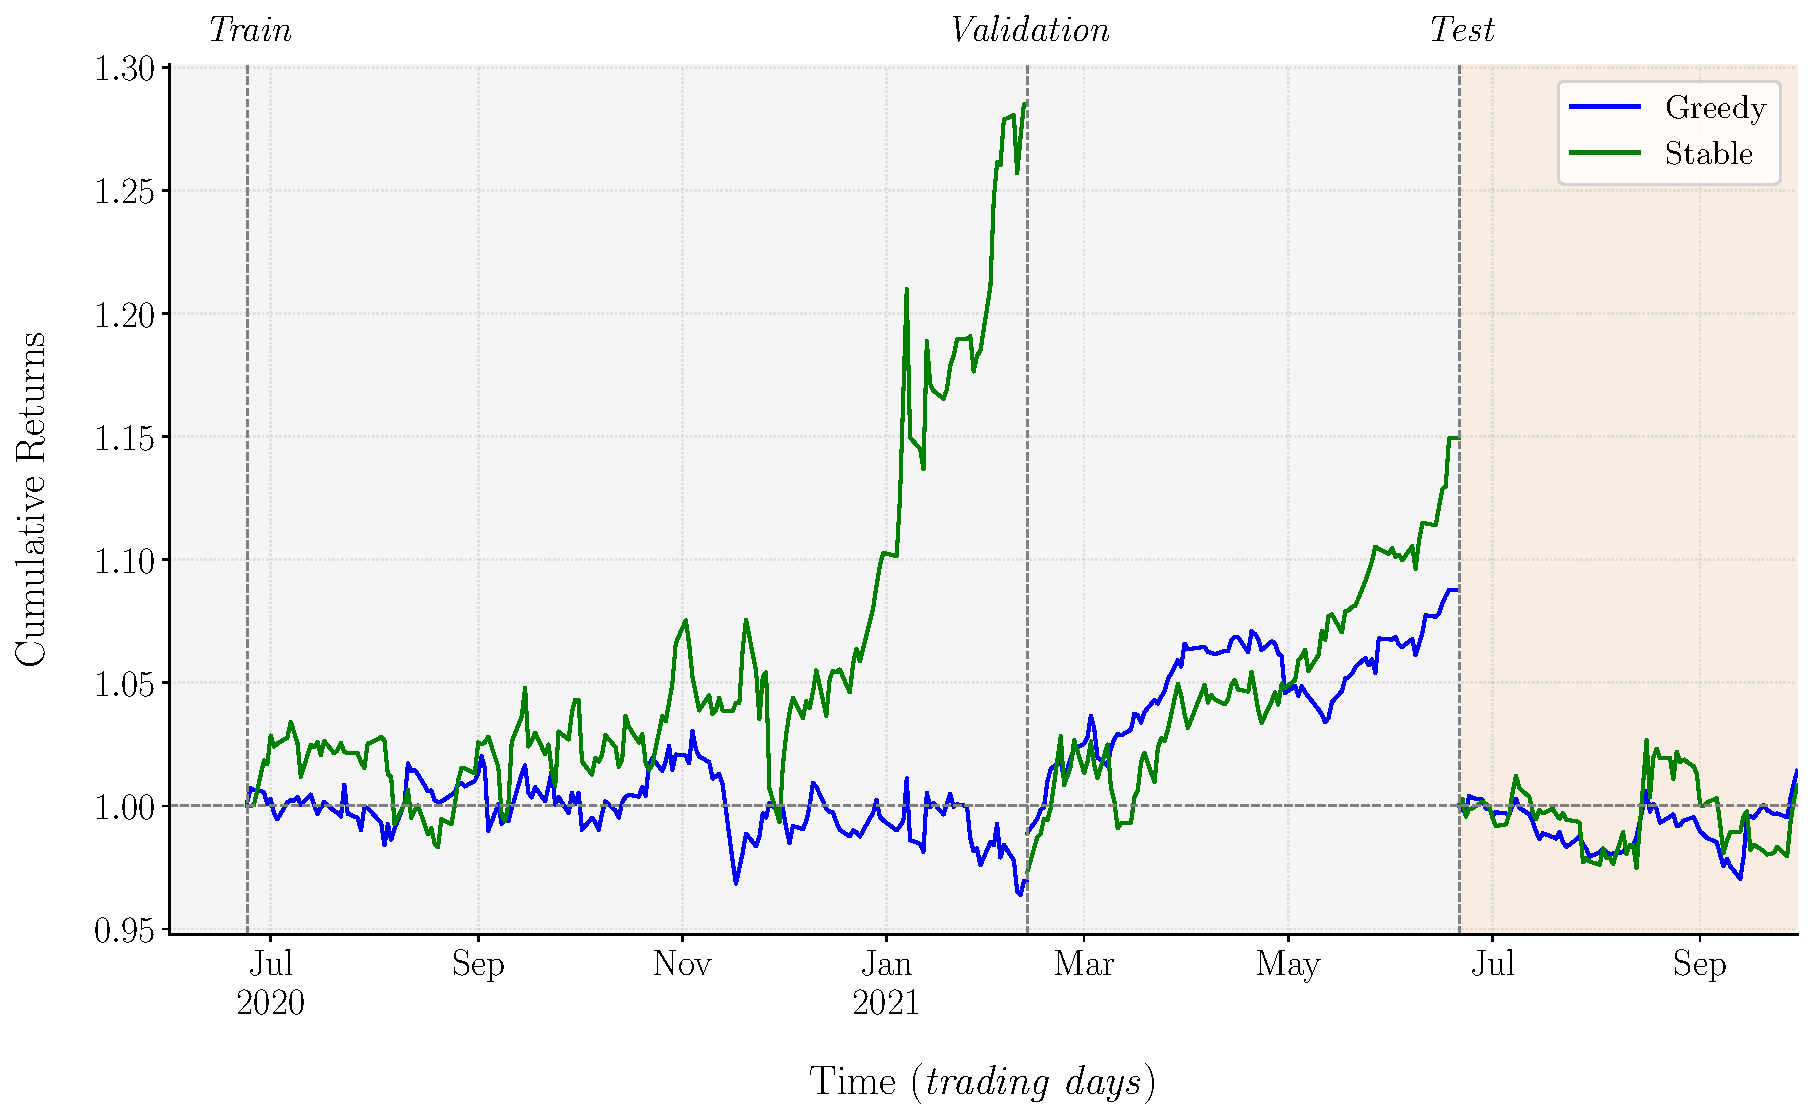
\includegraphics[scale=0.58]{/Users/jesusvillotamiranda/Library/CloudStorage/OneDrive-UniversidaddeLaRioja/CEMFI/__MSc__/__Second_year__/6th_Term/MasterThesis/__Output/KMeans_Portfolio_Cum_Returns_(L=4,theta=0.5k).pdf}
  \subcaption*{\textit{Note: The holding period of the beta-neutral strategies is set to $L$ = 4 trading days and the number of traded clusters is, $\theta = \integer{0.5k}=13$ as we have $k^*=26$ clusters. The selection criteria for these parameters is based on maximizing the Sharpe Ratios of the train and validation samples.}}
  \label{fig:KMeans_Portfolio_Cum_Returns}
\end{figure}
%----------------------------------------------------


%\red{The correlation between the trading signals generated by the greedy and stable algorithms is 0.512450. What is the correlation in each data split?
%}



%----------------------------------------------------
\inserthere{tab:KMeans_portfolio_statistics}

\begin{table}[H]
    \caption{Statistics of $\mathcal{P}_{\t{KMeans}}$ across data splits}
    \centering
    \renewcommand{\arraystretch}{0.8}
%    \begin{tabular}{|c|c|c|c|c|c|}
    \begin{tabular}{cccccc}
    	\hline \Xhline{2\arrayrulewidth}
%        \rowcolor{gray!10}
        \textbf{Split} & \textbf{Algorithm} & \textbf{Cum. Return} & \textbf{Avg. Return} & \textbf{St. Deviation} & \textbf{Sharpe Ratio} \\
%        \rowcolor{gray!10}
        & & & \textit{(daily)} & \textit{(daily)} & \textit{(annual)} \\
        \hline \Xhline{2\arrayrulewidth}
        \multirow{2}{*}{All}       & \textit{Greedy} & 1.070 & 0.021 & 0.006 & 0.54 \\        & \textit{Stable} & 1.489 & 0.121 & 0.011 & 1.82 \\         \hline          \multirow{2}{*}{Train}       & \textit{Greedy} & 0.969 & -0.019 & 0.007 & -0.41 \\        & \textit{Stable} & 1.285 & 0.151 & 0.012 & 1.97 \\         \hline          \multirow{2}{*}{Validation}       & \textit{Greedy} & 1.088 & 0.094 & 0.005 & 3.23 \\        & \textit{Stable} & 1.149 & 0.155 & 0.008 & 2.93 \\         \hline          \multirow{2}{*}{Test}       & \textit{Greedy} & 1.014 & 0.019 & 0.004 & 0.70 \\        & \textit{Stable} & 1.008 & 0.011 & 0.009 & 0.20 \\         \hline \Xhline{2\arrayrulewidth}
    \end{tabular}
    \label{tab:KMeans_portfolio_statistics}
\vspace{0.5cm}
\subcaption*{\textit{Note: Portfolio statistics of the trading strategy based on clusters obtained from applying KMeans to article embeddings. The statistics provided are: Cumulative Return, Average Return, Standard Deviation and Sharpe Ratio, which have been computed in accordance to the formulas provided in the text. Such statistics are provided for both cluster-selection algorithms: Greedy and Stable. The Greedy algorithm longs (shorts) clusters that maximize (minimize) the cluster-average-$SR$ in the validation sample subject to a positivity (negativity) constraint, while the Stable algorithm longs (shorts) clusters that minimize the rank difference between the training and validation rankings of the cluster-average-$SR$'s subject to a positivity (negativity) constraint, which is now imposed on both sample splits. In both algorithms, the cardinality of each leg is upper-bounded by a hyperparameter $\theta$. 
The holding period of the beta-neutral positions is set to $L$ = 4 trading days and the number of traded clusters is, $\theta = 0.5k=13$ as there are $k^*=26$ KMeans clusters of article embeddings. The selection criteria for these hyperparameters ($L,\theta$) is based on maximizing the Sharpe Ratios of the train and validation samples.
} }
\end{table}
%----------------------------------------------------


